\documentclass[12pt,a4paper]{report}
\usepackage{iftex}
\ifPDFTeX
  \usepackage[utf8]{inputenc}
  \usepackage[T5]{fontenc}
  \usepackage[vietnamese]{babel}
  \usepackage{mathptmx}
\else
  \usepackage{fontspec}
  \setmainfont{Tinos}
  \setsansfont{Arimo}
  \setmonofont{Liberation Mono}[Scale=0.88]
  \usepackage[vietnamese,provide=*]{babel}
\fi
\usepackage{graphicx}
\usepackage{amsmath,amssymb}
\usepackage{booktabs}
\usepackage{multirow}
\usepackage[colorlinks=true,linkcolor=black,citecolor=black,urlcolor=blue]{hyperref}
\usepackage{caption}
\usepackage{subcaption}
\usepackage{float}
\usepackage{listings}
\usepackage[ruled,vlined]{algorithm2e}
\usepackage[left=3cm,right=2cm,top=2cm,bottom=2cm]{geometry}
\usepackage{setspace}
\usepackage{titlesec}
\usepackage[nottoc]{tocbibind}
\usepackage{titletoc}
\newcommand{\tocchapname}{CHƯƠNG}
\titlecontents{chapter}[0pt]{\addvspace{8pt}\bfseries}{\tocchapname~\thecontentslabel.\enspace}{}{\titlerule*[0.6pc]{.}\contentspage}
\usepackage{fancyhdr}
\usepackage{tikz}
\usetikzlibrary{calc,arrows.meta,positioning,shapes.geometric,shapes.multipart,fit,backgrounds}
\usepackage{pgfplots}
\pgfplotsset{compat=1.18}
\usepackage{longtable}
\usepackage{tabularx}
\usepackage{xcolor}
\usepackage{indentfirst}

\usepackage{scrextend}
\changefontsizes{13pt}

\definecolor{codebg}{RGB}{246,248,250}
\lstset{
  basicstyle=\ttfamily\footnotesize,
  backgroundcolor=\color{codebg},
  breaklines=true,
  frame=single,
  rulecolor=\color{black!25},
  columns=fullflexible,
  keepspaces=true,
  showstringspaces=false,
  extendedchars=true,
  inputencoding=utf8
}

\setlength{\headheight}{16pt}
\pagestyle{fancy}
\fancyhf{}
\fancyhead[C]{\thepage}
\renewcommand{\headrulewidth}{0pt}
\fancyfoot{}

\fancypagestyle{plain}{
  \fancyhf{}
  \fancyhead[C]{\thepage}
  \renewcommand{\headrulewidth}{0pt}
  \fancyfoot{}
}

\addto\captionsvietnamese{
  \renewcommand{\figurename}{Hình}
  \renewcommand{\tablename}{Bảng}
  \renewcommand{\chaptername}{CHƯƠNG}
  \renewcommand{\contentsname}{MỤC LỤC}
  \renewcommand{\listfigurename}{DANH MỤC HÌNH VẼ}
  \renewcommand{\listtablename}{DANH MỤC BẢNG BIỂU}
  \renewcommand{\bibname}{TÀI LIỆU THAM KHẢO}
  \renewcommand{\appendixname}{PHỤ LỤC}
}

\setstretch{1.3}
\raggedbottom
\setlength{\parskip}{\medskipamount}
\setcounter{secnumdepth}{3}
\setcounter{tocdepth}{3}

\titleformat{\chapter}[block]
  {\normalfont\fontsize{13pt}{15.6pt}\selectfont\bfseries\centering}
  {\MakeUppercase{\chaptertitlename}\ \thechapter:}{0.5em}{\MakeUppercase}
\titlespacing*{\chapter}{0pt}{-20pt}{20pt}

\titleformat{name=\chapter,numberless}[block]
  {\normalfont\fontsize{13pt}{15.6pt}\selectfont\bfseries\centering}
  {}{0pt}{\MakeUppercase}

\newcommand{\specialchapter}[1]{
  \chapter*{#1}
  \addcontentsline{toc}{chapter}{#1}
  \markboth{#1}{#1}
}

\titleformat{\section}{\normalfont\fontsize{13pt}{15.6pt}\selectfont\bfseries}{\thesection.}{0.5em}{\MakeUppercase}
\titleformat{\subsection}{\normalfont\fontsize{13pt}{15.6pt}\selectfont\bfseries}{\thesubsection.}{0.5em}{}
\titleformat{\subsubsection}{\normalfont\fontsize{13pt}{15.6pt}\selectfont\itshape}{\thesubsubsection.}{0.5em}{}

\newcommand{\truong}{ĐẠI HỌC PHENIKAA}
\newcommand{\loaibaocao}{BÁO CÁO ĐỒ ÁN}
\newcommand{\tendaitai}{Hệ thống tìm kiếm sản phẩm thời trang\\đa mô thức bằng truy vấn tiếng Việt\\và hình ảnh}
\newcommand{\tendaitaien}{Multimodal Fashion Product Search}
\newcommand{\linhvuc}{Trí tuệ nhân tạo, Truy hồi thông tin đa mô thức}
\newcommand{\chuyennganh}{Khoa học máy tính}
\newcommand{\hocphan}{Mạng nơron và học sâu-1-3-25(N01)}
\newcommand{\gvhd}{PGS. TS. Phạm Tiến Lâm}
\newcommand{\thoigian}{Hà Nội, tháng 10 năm 2026}

\newcommand{\bia}[1]{
\begin{titlepage}
\begin{tikzpicture}[remember picture, overlay]
    \draw[line width = 2pt] ($(current page.north west) + (3cm,-2cm)$) rectangle ($(current page.south east) + (-2cm,2cm)$);
\end{tikzpicture}
\begin{center}
    {\fontsize{13pt}{15.6pt}\selectfont BỘ GIÁO DỤC VÀ ĐÀO TẠO} \\
    {\fontsize{13pt}{15.6pt}\selectfont \textbf{\truong}} \\
    \vspace{0.1cm}
    \rule{6cm}{1.2pt} \\
    #1
    \vspace{1.2cm}
    {\fontsize{22pt}{26pt}\selectfont \textbf{\loaibaocao}} \\
    \vspace{1.2cm}
    {\fontsize{16pt}{19.2pt}\selectfont \textbf{TÊN ĐỀ TÀI:}} \\
    \vspace{0.6cm}
    \parbox{0.86\textwidth}{\centering\fontsize{15pt}{20pt}\selectfont \textbf{\MakeUppercase{\tendaitai}}} \\
    \vspace{0.3cm}
    {\fontsize{13pt}{15.6pt}\selectfont \textit{(\tendaitaien)}} \\
    \vspace{1.2cm}
\begin{flushleft}
    \hspace{2cm} \fontsize{13pt}{15.6pt}\selectfont Sinh viên thực hiện: \textbf{Lê Bảo Hưng - 23010090} \\
    \hspace{2cm} \fontsize{13pt}{15.6pt}\selectfont \phantom{Sinh viên thực hiện: } \textbf{Đinh Việt Hoàng - 23010051} \\
    \hspace{2cm} \fontsize{13pt}{15.6pt}\selectfont \phantom{Sinh viên thực hiện: } \textbf{Nguyễn Trung Hiếu - 23011098} \\ [0.3cm]
\end{flushleft}
\begin{center}
    \vspace{0.5cm}
    \fontsize{13pt}{15.6pt}\selectfont Học phần: \textbf{\hocphan}\\
    \vspace{0.5cm}
    \fontsize{13pt}{15.6pt}\selectfont Giảng viên hướng dẫn: \textbf{\gvhd}
\end{center}
    \vfill
    {\fontsize{13pt}{15.6pt}\selectfont \textbf{\thoigian}}
\end{center}
\end{titlepage}
}

\begin{document}

\bia{\vspace{1.2cm}
\includegraphics[width=6cm]{graphics/logo_phenikaa.png}\\}
\bia{\vspace{2cm}}

\pagenumbering{roman}
\tableofcontents
\newpage
\listoffigures
\newpage
\listoftables
\newpage
\chapter*{DANH MỤC CÁC TỪ VIẾT TẮT}
\addcontentsline{toc}{chapter}{DANH MỤC CÁC TỪ VIẾT TẮT}

\begingroup
\footnotesize
\renewcommand{\arraystretch}{0.92}
\newcolumntype{L}[1]{>{\raggedright\arraybackslash}p{#1}}
\begin{longtable}{@{}L{2.3cm}L{5.9cm}L{6.8cm}@{}}
\toprule
\textbf{Viết tắt} & \textbf{Tiếng Anh} & \textbf{Ý nghĩa} \\
\midrule
\endfirsthead
\toprule
\textbf{Viết tắt} & \textbf{Tiếng Anh} & \textbf{Ý nghĩa} \\
\midrule
\endhead
\bottomrule
\endfoot
API & Application Programming Interface & Giao diện lập trình ứng dụng \\
BEIR & Benchmarking Information Retrieval & Bộ chuẩn đánh giá tìm kiếm thông tin \\
bf16, fp32 & Brain float 16-bit; float 32-bit & Số thực dấu phẩy động 16 bit và 32 bit \\
BM25 & Best Matching 25 & Hàm xếp hạng văn bản theo từ khoá \\
CH & -- & Câu hỏi nghiên cứu \\
CLIP & Contrastive Language-Image Pre-training & Huấn luyện chung ảnh và văn bản bằng hàm mất mát tương phản \\
CPU & Central Processing Unit & Bộ xử lý trung tâm \\
CSV & Comma-Separated Values & Bảng văn bản, ngăn cách bằng dấu phẩy \\
CUDA & Compute Unified Device Architecture & Nền tảng tính toán song song trên GPU \\
DCG, IDCG & Discounted Cumulative Gain; Ideal DCG & Độ lợi tích luỹ có chiết khấu; bản lý tưởng \\
DoRA & Weight-Decomposed Low-Rank Adaptation & Tinh chỉnh hạng thấp, tách độ lớn và hướng \\
FR, NFR & Functional Requirement; Non-Functional Requirement & Yêu cầu chức năng; yêu cầu phi chức năng \\
GPU & Graphics Processing Unit & Bộ xử lý đồ hoạ \\
HNSW & Hierarchical Navigable Small World & Đồ thị nhiều tầng tìm láng giềng gần đúng \\
IDF & Inverse Document Frequency & Nghịch đảo tần suất tài liệu \\
JSON, JSONL & JavaScript Object Notation; JSON Lines & Định dạng dữ liệu văn bản dạng khoá--giá trị; JSONL: mỗi dòng một đối tượng JSON \\
KNN & K-Nearest Neighbors & K láng giềng gần nhất \\
KT & -- & Hạng mục kiểm thử \\
LoRA & Low-Rank Adaptation & Tinh chỉnh bằng ma trận hạng thấp \\
MRR & Mean Reciprocal Rank & Trung bình nghịch đảo hạng đúng đầu tiên \\
NaN & Not a Number & Giá trị không phải số \\
nDCG & Normalized Discounted Cumulative Gain & Độ lợi tích luỹ chiết khấu đã chuẩn hoá \\
NFC & Normalization Form C & Dạng chuẩn hoá Unicode có ghép ký tự \\
OT & Optimal Transport & Vận chuyển tối ưu, phần tên của ViSigLIP-OT \\
p50, p95 & 50th, 95th percentile & Phân vị thứ 50 và thứ 95 của độ trễ \\
pHash & Perceptual Hash & Mã băm cảm nhận, dùng để lọc ảnh trùng \\
ResNet & Residual Network & Mạng tích chập có kết nối phần dư \\
SigLIP & Sigmoid Loss for Language-Image Pre-training & Huấn luyện chung ảnh và văn bản bằng hàm mất mát sigmoid \\
TLS & Transport Layer Security & Giao thức mã hoá đường truyền \\
UC & Use Case & Chức năng (chỉ giữ trong tên sơ đồ UML) \\
UUID & Universally Unique Identifier & Định danh duy nhất dạng 128 bit \\
ViT & Vision Transformer & Mô hình Transformer cho ảnh \\
\end{longtable}
\endgroup

\newpage
\pagenumbering{arabic}
\chapter*{MỞ ĐẦU}
\addcontentsline{toc}{chapter}{MỞ ĐẦU}

Người tìm đồ thời trang thường mô tả thứ mình muốn bằng màu sắc, dáng áo và phong cách, ít khi gọi đúng tên sản phẩm. Tìm kiếm theo từ khoá chỉ khớp khi câu truy vấn và văn bản mô tả dùng cùng từ. Với tiếng Việt, khó khăn tăng lên vì cách nói về thời trang trộn từ thuần Việt, từ mượn tiếng Anh và từ mới. Một hướng khác là tìm thẳng trên ảnh, dùng các mô hình học chung biểu diễn của ảnh và văn bản.

Đồ án xây dựng một hệ thống tìm ảnh sản phẩm thời trang bằng truy vấn tiếng Việt, rồi đo xem mô hình biểu diễn chung nào cho kết quả tốt hơn BM25, phương pháp xếp hạng theo từ khoá, và chênh bao nhiêu. Mỗi ảnh trong catalog được mã hoá thành vector một lần; khi tìm, câu truy vấn được mã hoá vào cùng không gian và hệ thống lấy các ảnh có vector gần nhất. Ba mô hình dùng sẵn là CLIP, SigLIP~2 và ViSigLIP-OT được đối chiếu với BM25. Sau đó nhóm tinh chỉnh SigLIP~2 bằng DoRA, một phương pháp chỉ huấn luyện một phần nhỏ tham số bổ sung.

Đánh giá dùng ảnh công khai của Fashionpedia và một bộ 155 truy vấn tiếng Việt tự soạn; mỗi mô hình được so với BM25 bằng kiểm định bootstrap ghép cặp. Vì nhãn do người chấm và một bộ lọc tự động gán nên có thể sai, nhóm rà lại từng truy vấn mà mô hình trả sai ở top-10 để xác định lỗi thuộc về mô hình hay về nhãn. Báo cáo gồm năm chương: Chương~\ref{chap:tong_quan} đặt bài toán, mục tiêu và phạm vi; Chương~\ref{chap:co_so_ly_thuyet} điểm lại cơ sở lý thuyết; Chương~\ref{chap:thiet_ke} và \ref{chap:cai_dat} trình bày thiết kế và cài đặt; Chương~\ref{chap:danh_gia} nêu kết quả đo, phân tích lỗi và trả lời các câu hỏi nghiên cứu.


\chapter{Tổng quan}
\label{chap:tong_quan}

Chương này đặt bài toán, mục tiêu và ba câu hỏi nghiên cứu của đồ án, rồi nêu phạm vi, đóng góp và bố cục báo cáo.

\section{Bối cảnh và vấn đề}
\label{sec:boi-canh}

Một món đồ thời trang được nhận ra qua hình dáng, màu sắc, chất liệu và phong cách; những thuộc tính này dễ thấy bằng mắt nhưng khó gọi đúng tên. Người tìm đồ thường chỉ có một hình dung như ``đầm y2k dáng ôm màu hồng'' hay ``áo bomber jacket dáng ngắn'', chứ không biết người bán đặt tên sản phẩm là gì. Ô tìm kiếm theo từ khoá xử lý tình huống này kém. BM25~\cite{robertson2009bm25} chỉ xếp hạng cao một văn bản khi văn bản đó dùng đúng các từ có trong truy vấn, nên gặp hiện tượng lệch từ vựng giữa người hỏi và người mô tả~\cite{manning2008ir}.

Các mô hình học biểu diễn chung cho ảnh và văn bản đưa ra một cách khác. CLIP~\cite{radford2021clip}, SigLIP~\cite{zhai2023siglip} và SigLIP~2~\cite{tschannen2025siglip2} đặt ảnh và câu mô tả vào cùng một không gian vector, nên một câu truy vấn có thể so trực tiếp với ảnh sản phẩm mà không cần văn bản mô tả sản phẩm. FashionCLIP~\cite{chia2022fashionclip} đã áp dụng hướng này cho thời trang. Các mô hình này được huấn luyện với tiếng Việt ở mức rất khác nhau: CLIP không nhắm tới tiếng Việt, SigLIP~2 là mô hình đa ngữ, còn ViSigLIP-OT~\cite{viclipot2026} được huấn luyện riêng cho tiếng Việt. Chúng xử lý đến đâu những cách nói đời thường như ``áo croptop'' hay ``quần wide leg'' thì chưa có số đo trên dữ liệu thời trang tiếng Việt. Đồ án đặt mục tiêu đo điều đó.

Bài toán gặp ba khó khăn cụ thể.

\begin{itemize}
    \item \textbf{Từ vựng đời thường:} truy vấn tiếng Việt về thời trang trộn từ thuần Việt, từ mượn tiếng Anh và từ mới, như ``giày sneaker trắng basic'' hay ``áo croptop rib bo sát người''. Mô hình chỉ khớp theo từ sẽ trượt khi từ trong truy vấn không trùng với từ trong văn bản của sản phẩm.
    \item \textbf{Thiếu bộ đánh giá:} Fashionpedia~\cite{jia2020fashionpedia} được xây dựng cho phát hiện và phân đoạn nên không có truy vấn hay nhãn cho bài toán tìm kiếm. Phần điểm lại nghiên cứu ở Chương~\ref{chap:co_so_ly_thuyet} cũng không tìm thấy bộ truy vấn tiếng Việt nào cho tìm ảnh thời trang. Muốn so sánh các mô hình thì nhóm phải tự soạn truy vấn và tự gán nhãn.
    \item \textbf{Ảnh người mặc cả bộ:} mỗi ảnh trong catalog chứa trung bình 2,95 món, trong khi catalog chỉ lưu một danh mục chính cho mỗi ảnh. Với truy vấn về kính, giày hay túi, không có ảnh sản phẩm đứng riêng, nên khó nói thế nào là một kết quả đúng.
\end{itemize}

\section{Mục tiêu}
\label{sec:muc-tieu}

Đồ án xây dựng một hệ thống tìm ảnh sản phẩm thời trang bằng truy vấn tiếng Việt. Trên một bộ đánh giá riêng, hệ thống được đối chiếu với BM25 chạy trên tên danh mục của ảnh. Mô hình được dùng theo hai cách: giữ nguyên bản đã huấn luyện sẵn (zero-shot) hoặc tinh chỉnh thêm trên dữ liệu của đồ án. Năm mục tiêu cụ thể gồm:

\begin{enumerate}
    \item Dựng catalog tìm kiếm gồm 6.963 ảnh Fashionpedia (tập kiểm tra sau khi lọc trùng và chia 70/15/15 với seed 42), tách khỏi dữ liệu tinh chỉnh.
    \item Soạn 155 truy vấn tiếng Việt chia thành bốn nhóm và gán nhãn theo thang 0/1/2. Người chấm độc lập gán một phần nhãn; độ đồng thuận giữa họ được đo bằng hệ số $\kappa$ của Cohen. Phần còn lại được gán nhãn 0 bằng bộ lọc tự động (Mục~\ref{sec:du-lieu-cach-do}).
    \item So sánh năm hệ trên cùng 155 truy vấn bằng Recall@1, Recall@5, Recall@10, MRR và nDCG@10, kèm kiểm định bootstrap ghép cặp 10.000 lần.
    \item Tinh chỉnh SigLIP~2 bằng DoRA với hạng (rank) bằng 8, rồi so với SigLIP~2 gốc, với LoRA thường, và với cấu hình không dùng mẫu âm khó (hard negative, tức ảnh sai nhưng rất giống ảnh đúng).
    \item Xây dựng API và giao diện web truy vấn trên Qdrant với catalog 6.963 ảnh. Độ trễ mã hoá và tìm kiếm của từng truy vấn được đo riêng ở bước suy luận và so với chỉ tiêu dưới 200~ms của đề cương.
\end{enumerate}

\section{Câu hỏi nghiên cứu}
\label{sec:cau-hoi-nghien-cuu}

Ba câu hỏi nghiên cứu được trả lời bằng số liệu ở Mục~\ref{sec:tra-loi-ch}. Bảng~\ref{tab:ch1-cau-hoi} cho biết mỗi câu so sánh những hệ nào.

\begin{description}
    \item[CH1.] Tìm kiếm bằng biểu diễn chung đa mô thức dùng zero-shot (SigLIP~2, CLIP, ViSigLIP-OT) có tốt hơn BM25 trên truy vấn tiếng Việt không?
    \item[CH2.] Tinh chỉnh SigLIP~2 bằng adapter có cho kết quả tốt hơn zero-shot, xét theo kiểm định ghép cặp, hay không? Nếu có, DoRA và mẫu âm khó có làm kết quả tốt hơn LoRA thường hay không?
    \item[CH3.] Nguyên nhân lỗi còn lại nằm ở mô hình hay ở nhãn và catalog?
\end{description}

\begin{table}[H]
\centering
\caption{Câu hỏi nghiên cứu và đối tượng so sánh}
\label{tab:ch1-cau-hoi}
\small
\renewcommand{\arraystretch}{1.12}
\begin{tabularx}{\textwidth}{@{}l >{\raggedright\arraybackslash}X >{\raggedright\arraybackslash}p{3.6cm}@{}}
\toprule
\textbf{Câu} & \textbf{Đối tượng so sánh} & \textbf{Nơi trả lời} \\
\midrule
CH1 & SigLIP~2, CLIP và ViSigLIP-OT so với BM25 & Mục~\ref{sec:so-sanh-cau-hinh}, \ref{sec:kiem-dinh} \\
CH2 & SigLIP~2 tinh chỉnh so với SigLIP~2 gốc; DoRA so với LoRA thường; có và không có mẫu âm khó & Mục~\ref{sec:ablation}, \ref{sec:kiem-dinh}, \ref{sec:danh-gia-dau-ra} \\
CH3 & Các truy vấn mà hệ DoRA trượt ở top-10 & Mục~\ref{sec:tra-loi-ch}, dựa trên Mục~\ref{sec:doi-soat-nhan} \\
\bottomrule
\end{tabularx}
\end{table}

\section{Phạm vi và phương pháp}
\label{sec:pham-vi}

Dữ liệu là Fashionpedia, một bộ ảnh người mặc công khai với 46 danh mục. Sau khi lọc trùng còn 46.416 ảnh, chia thành 32.491 ảnh huấn luyện, 6.962 ảnh xác thực và 6.963 ảnh kiểm tra; catalog dùng để tìm kiếm và đánh giá là tập kiểm tra. Catalog không có màu, chất liệu, giá hay mô tả của người bán, chỉ có tên các danh mục có trong ảnh. Vì vậy BM25 trong đồ án chạy trên tên danh mục, một văn bản ngắn và ít thông tin, nên là đối chứng yếu hơn một ô tìm kiếm có thêm mô tả của người bán. Truy vấn là văn bản tiếng Việt, ảnh là đối tượng được tìm.

Bảng~\ref{tab:ch1-he-thong} liệt kê các hệ được đo. Năm hệ đầu có nhãn đầy đủ cho top-10 và tạo thành bảng kết quả chính. Ba hệ sau chỉ dùng để khảo sát loại bỏ thành phần (ablation), không nằm trong tập ứng viên chấm nhãn nên nhãn của chúng chưa đầy đủ. Riêng ViSigLIP-OT phải chạy trên CPU vì trên GPU mô hình cho giá trị NaN (không phải số), nên điểm thấp của hệ này có thể một phần do cách chạy, không hoàn toàn do chất lượng biểu diễn.

\begin{table}[H]
\centering
\caption{Các hệ được đo}
\label{tab:ch1-he-thong}
\small
\renewcommand{\arraystretch}{1.12}
\begin{tabularx}{\textwidth}{@{}>{\raggedright\arraybackslash}p{4.3cm} >{\raggedright\arraybackslash}X c l@{}}
\toprule
\textbf{Hệ} & \textbf{Cách biểu diễn} & \textbf{Số chiều vector} & \textbf{Dùng trong} \\
\midrule
BM25 & Tìm theo từ khoá; văn bản của sản phẩm là tên các danh mục & -- & Bảng chính \\
CLIP ViT-B/32 & Biểu diễn chung ảnh--văn bản, zero-shot & 512 & Bảng chính \\
SigLIP~2 (hệ gốc) & Biểu diễn chung ảnh--văn bản đa ngữ, zero-shot & 768 & Bảng chính \\
ViSigLIP-OT & Biểu diễn chung cho tiếng Việt, zero-shot & 768 & Bảng chính \\
SigLIP~2 + DoRA (hệ DoRA) & SigLIP~2 tinh chỉnh, có mẫu âm khó & 768 & Bảng chính \\
SigLIP~1 & Biểu diễn chung ảnh--văn bản, zero-shot & 768 & Ablation \\
SigLIP~2 + LoRA thường & Tinh chỉnh không dùng DoRA & 768 & Ablation \\
SigLIP~2 + DoRA, không mẫu âm khó & Tinh chỉnh chỉ với mẫu âm lấy từ các ảnh khác trong cùng mỗi lô huấn luyện & 768 & Ablation \\
\bottomrule
\end{tabularx}
\end{table}

Vì chưa có nhãn sẵn, nhóm tự dựng bộ đánh giá. Tập ứng viên gồm 10 kết quả đầu của BM25, CLIP, SigLIP~2 và ViSigLIP-OT (vòng chấm thứ nhất) và của hệ DoRA (vòng thứ hai); các kết quả được xáo trộn và ẩn tên hệ trước khi chấm. Ba cấu hình ablation không vào tập này. Mỗi cặp do người chấm xem có hai người chấm độc lập, riêng 296 cặp có ba người; các cặp còn lại do bộ lọc tự động gán điểm 0 (Mục~\ref{sec:du-lieu-cach-do}). Chất lượng đo bằng Recall@$K$, MRR và nDCG@10; chênh lệch giữa hai hệ được kiểm định bằng bootstrap ghép cặp theo truy vấn. Độ trễ đo từng truy vấn một.

Phạm vi đánh giá có các giới hạn sau.

\begin{itemize}
    \item \textbf{Loại truy vấn:} đồ án đánh giá truy vấn bằng văn bản. Tìm bằng ảnh nằm ngoài phạm vi đánh giá.
    \item \textbf{Giới hạn của bộ truy vấn:} bộ truy vấn không dựa trên dữ liệu thương mại hay khảo sát người dùng. Bộ không có câu nào về áo dài, áo bà ba hay nón lá, nên báo cáo không kết luận về thị trường hay độ lệch văn hoá.
    \item \textbf{Khảo sát loại bỏ thành phần:} gồm bốn trong bảy trục dự kiến; ba trục còn lại dành cho giai đoạn sau. Mỗi cấu hình huấn luyện một lần với seed 42.
    \item \textbf{Vận hành thực tế:} độ trễ qua API web và kho vector, độ chính xác của chỉ mục gần đúng và khả năng chịu tải đồng thời là hướng phát triển. Mục~\ref{sec:han-che-danh-gia} tổng hợp các giới hạn này.
\end{itemize}

\section{Đóng góp}
\label{sec:dong-gop}

Đồ án có bốn đóng góp, mỗi đóng góp gắn với một kết quả được trình bày ở Chương~\ref{chap:danh_gia}.

\begin{enumerate}
    \item \textbf{Bộ đánh giá tiếng Việt cho tìm ảnh thời trang.} Bộ gồm 155 truy vấn chia bốn nhóm và 7.324 cặp (truy vấn, ảnh) có nhãn. Người chấm gán 4.951 cặp với $\kappa$ từ 0,44 đến 0,52; 2.373 cặp còn lại (khoảng một phần ba) do bộ lọc tự động gán 0.
    \item \textbf{So sánh có kiểm định giữa các hướng tìm kiếm.} SigLIP~2 gốc tốt hơn BM25 ở Recall@10 (0,865 so với 0,568); CLIP và ViSigLIP-OT thì không. Tinh chỉnh nâng Recall@1 từ 0,490 lên 0,697, nhưng mức tăng chưa quy được riêng cho DoRA hay mẫu âm khó.
    \item \textbf{Đối soát nhãn tự động.} Bộ lọc tự động gán 0 cho một phần cặp nhãn và làm lệch 35 truy vấn; khi rà lại, nhóm xác nhận 26 truy vấn trong số đó bị chấm sai. Cả 18 truy vấn mà hệ DoRA trượt ở top-10 đều thuộc 26 truy vấn này. Bảng chính vẫn tính trên đủ 155 truy vấn; việc bỏ 35 truy vấn chỉ nhằm xem độ nhạy (Mục~\ref{sec:doi-soat-nhan}, \ref{sec:sau-sua-loc}).
    \item \textbf{Kiến trúc dễ thay thành phần.} Hệ thống theo kiến trúc lục giác (cổng và bộ chuyển đổi). Phần lõi chỉ khai báo bốn cổng. Mô hình, kho vector và bộ tính chỉ số là các bộ chuyển đổi thay thế được, chọn bằng cấu hình. Nhờ đó đổi giữa CLIP, SigLIP~2 và ViSigLIP-OT, hay giữa kho trong bộ nhớ và Qdrant, không phải sửa lõi.
\end{enumerate}

\section{Bố cục báo cáo}
\label{sec:bo-cuc}

Chương~\ref{chap:co_so_ly_thuyet} điểm lại các nghiên cứu liên quan và khái niệm nền tảng. Chương~\ref{chap:thiet_ke} trình bày yêu cầu và thiết kế hệ thống; Chương~\ref{chap:cai_dat} mô tả cài đặt, các tham số chính, API web và giao diện web. Chương~\ref{chap:danh_gia} trình bày kế hoạch kiểm thử, kết quả đo, phân tích lỗi, đối soát nhãn và câu trả lời cho ba câu hỏi nghiên cứu. Phần Kết luận tóm tắt kết quả, hạn chế và hướng phát triển. Phụ lục~\ref{app:truy-van} và Phụ lục~\ref{app:doi-soat} liệt kê bộ truy vấn đánh giá và các truy vấn bị đánh dấu khi đối soát nhãn chấm 0 tự động.

\chapter{Cơ sở lý thuyết}
\label{chap:co_so_ly_thuyet}

Chương này điểm lại các hướng nghiên cứu gần với đề tài (Mục~\ref{sec:nghien-cuu-lien-quan}), rồi trình bày các khái niệm nền tảng (Mục~\ref{sec:khai-niem-nen-tang}) mà Chương~\ref{chap:thiet_ke} đến Chương~\ref{chap:danh_gia} sử dụng. Đó là biểu diễn chung ảnh và văn bản, hàm mất mát tương phản, BM25, tìm kiếm vector gần đúng, tinh chỉnh hiệu quả tham số và các chỉ số đánh giá.

\section{Các nghiên cứu liên quan}
\label{sec:nghien-cuu-lien-quan}

\textbf{Học biểu diễn ảnh và văn bản.} Học tương phản bắt nguồn từ học metric~\cite{hadsell2006contrastive}, rồi được mở rộng sang dạng dùng nhiều mẫu âm (cặp không khớp) trong cùng một lô với InfoNCE~\cite{oord2018cpc} và SimCLR~\cite{chen2020simclr}. CLIP~\cite{radford2021clip} áp dụng cách này cho cặp ảnh và mô tả thu thập từ Internet: hai bộ mã hoá được huấn luyện chung để ảnh và câu mô tả của nó nằm gần nhau trong một không gian vector. CLIP vì thế tìm được ảnh theo câu mô tả mà không cần huấn luyện thêm trên miền đó (zero-shot). Bộ mã hoá ảnh thường là Vision Transformer~\cite{dosovitskiy2021vit}, bộ mã hoá văn bản là Transformer~\cite{vaswani2017attention}. Dense Passage Retrieval~\cite{karpukhin2020dpr} dùng cùng cấu trúc hai bộ mã hoá cho bài toán tìm kiếm văn bản.

\textbf{Hàm mất mát sigmoid.} SigLIP~\cite{zhai2023siglip} thay softmax trên cả lô của CLIP bằng sigmoid tính riêng cho từng cặp ảnh--văn bản, nên không cần chuẩn hoá trên toàn lô. SigLIP~2~\cite{tschannen2025siglip2} giữ hàm sigmoid, bổ sung các mục tiêu phụ về hiểu ngữ nghĩa và định vị, và được huấn luyện trên dữ liệu đa ngữ. Cùng họ kiến trúc, ViSigLIP-OT là mô hình ảnh--văn bản huấn luyện cho tiếng Việt, đi cùng công trình ViCLIP-OT~\cite{viclipot2026} và có trọng số công bố trên Hugging Face.

\textbf{Tìm kiếm thưa theo từ khoá.} BM25~\cite{robertson1994okapi,robertson2009bm25} xếp hạng văn bản theo tần suất xuất hiện của từ truy vấn và độ hiếm của từ đó trong tập tài liệu~\cite{sparckjones1972idf}. BM25 không cần huấn luyện và vẫn là mốc đối chứng mạnh trên nhiều miền khi các mô hình vector chưa được tinh chỉnh~\cite{thakur2021beir}. Hạn chế của nó là chỉ khớp được khi truy vấn và tài liệu dùng cùng một từ.

\textbf{Tìm kiếm gần đúng và tinh chỉnh hiệu quả tham số.} HNSW~\cite{malkov2020hnsw} xây đồ thị nhiều tầng để tìm láng giềng gần đúng (Mục~\ref{sec:tim-kiem-gan-dung}). LoRA~\cite{hu2022lora} và DoRA~\cite{liu2024dora} chỉ huấn luyện thêm một số ít tham số bên cạnh trọng số gốc (Mục~\ref{sec:tinh-chinh-ly-thuyet}).

\textbf{Huấn luyện tương phản với lô lớn và mẫu âm khó.} Hàm mất mát tương phản cần lô lớn mà bộ nhớ GPU có hạn, nên GradCache~\cite{gao2021gradcache} tách bước tính biểu diễn khỏi bước tính gradient để huấn luyện lô hiệu dụng lớn trên GPU nhỏ. Về dữ liệu, mẫu âm khó~\cite{robinson2021hardneg} cải thiện chất lượng biểu diễn học tương phản; ANCE~\cite{xiong2021ance} áp dụng ý tưởng này cho tìm kiếm văn bản bằng cách lấy mẫu âm từ chính chỉ mục đang huấn luyện.

\textbf{Biểu diễn cho thời trang.} FashionCLIP~\cite{chia2022fashionclip} tinh chỉnh CLIP trên ảnh sản phẩm kèm mô tả của một nhà bán lẻ, còn FashionViL~\cite{han2022fashionvil} huấn luyện riêng cho thời trang với các tác vụ ảnh--văn bản như tìm ảnh theo mô tả. Fashionpedia~\cite{jia2020fashionpedia} là bộ ảnh người mặc cả bộ trang phục, xây dựng cho phát hiện và phân đoạn chứ không cho tìm kiếm. Cả ba công trình đều dùng mô tả tiếng Anh.

\textbf{Mô hình ảnh--văn bản ngoài tiếng Anh.} Chinese-CLIP~\cite{yang2022chineseclip} huấn luyện lại CLIP trên cặp ảnh--văn bản tiếng Trung. M-CLIP~\cite{carlsson2022mclip} thay bộ mã hoá văn bản của CLIP bằng mô hình đa ngữ, giữ nguyên không gian của bộ mã hoá ảnh. Hai hướng này cho thấy hai cách đưa mô hình sang ngôn ngữ khác: huấn luyện lại toàn bộ và thay bộ mã hoá văn bản.

\textbf{Chỉ số đánh giá.} nDCG~\cite{jarvelin2002ndcg} cho phép chấm kết quả theo nhiều mức liên quan, còn Recall, MRR và các chỉ số thứ hạng khác được tổng hợp trong~\cite{manning2008ir}. BEIR~\cite{thakur2021beir} dùng nDCG@10 làm chỉ số chính. Khi so sánh hai hệ trên cùng tập truy vấn, kiểm định bootstrap~\cite{efron1993bootstrap} đánh giá độ chắc chắn của chênh lệch mà không giả định dạng phân phối. Cách đồ án áp dụng kiểm định này và giới hạn của nó nằm ở Mục~\ref{sec:chi-so-danh-gia}.

Các nghiên cứu nêu trên để lại hai khoảng trống. Thứ nhất, các mô hình thời trang chỉ dùng mô tả tiếng Anh, còn mô hình đa ngữ chưa được đo trên thời trang. Trong các nghiên cứu nhóm đã đọc, chưa có so sánh kiểm định thống kê giữa BM25, mô hình đa ngữ và mô hình huấn luyện riêng cho tiếng Việt. Thứ hai, nhóm chưa thấy bộ dữ liệu tìm kiếm thời trang có truy vấn và nhãn liên quan bằng tiếng Việt. Đồ án dựng bộ truy vấn và nhãn riêng, nêu rõ định nghĩa từng chỉ số, và kiểm định ghép cặp theo truy vấn cho các so sánh giữa các hệ.

Bảng~\ref{tab:so-sanh-nghien-cuu} tóm tắt các nghiên cứu theo bài toán, dữ liệu, ngôn ngữ và điểm khác với đề tài.

\begin{table}[H]
\centering
\caption{So sánh các nghiên cứu liên quan}
\label{tab:so-sanh-nghien-cuu}
\footnotesize
\begin{tabularx}{\textwidth}{@{}>{\raggedright\arraybackslash}p{2.7cm} >{\raggedright\arraybackslash}X >{\raggedright\arraybackslash}p{2.4cm} >{\raggedright\arraybackslash}p{1.5cm} >{\raggedright\arraybackslash}X@{}}
\toprule
\textbf{Nghiên cứu} & \textbf{Bài toán} & \textbf{Dữ liệu} & \textbf{Tiếng Việt} & \textbf{Điểm khác với đề tài} \\
\midrule
CLIP~\cite{radford2021clip} & Học biểu diễn ảnh--văn bản bằng softmax tương phản & Cặp ảnh--mô tả thu từ Internet & Không & Chỉ đo không tinh chỉnh, trên truy vấn tiếng Việt \\
SigLIP~\cite{zhai2023siglip}, SigLIP~2~\cite{tschannen2025siglip2} & Học biểu diễn ảnh--văn bản bằng sigmoid theo cặp & Dữ liệu web, SigLIP~2 đa ngữ & SigLIP~2: có (đa ngữ) & Tinh chỉnh SigLIP~2 bằng DoRA trên ảnh thời trang kèm tên danh mục tiếng Việt \\
ViSigLIP-OT~\cite{viclipot2026} & Học biểu diễn ảnh--văn bản cho tiếng Việt, họ SigLIP & Không rõ theo tài liệu công bố & Có & Đo không tinh chỉnh trên truy vấn thời trang \\
FashionCLIP~\cite{chia2022fashionclip} & Tinh chỉnh CLIP cho thời trang & Ảnh sản phẩm và mô tả của một nhà bán lẻ & Không & Truy vấn tiếng Việt; ảnh là người mặc cả bộ, không phải ảnh từng sản phẩm \\
FashionViL~\cite{han2022fashionvil} & Huấn luyện ảnh--văn bản riêng cho thời trang & Ảnh thời trang kèm mô tả tiếng Anh & Không & Truy vấn tiếng Việt; tự dựng bộ truy vấn và nhãn \\
Chinese-CLIP~\cite{yang2022chineseclip}, M-CLIP~\cite{carlsson2022mclip} & Đưa CLIP sang ngôn ngữ khác & Cặp ảnh--văn bản tiếng Trung; văn bản đa ngữ & Không & Đo trên truy vấn thời trang tiếng Việt \\
Fashionpedia~\cite{jia2020fashionpedia} & Phát hiện, phân đoạn, thuộc tính & Ảnh người mặc, 46 danh mục & Không & Dùng lại ảnh và bản thể cho tìm kiếm; tự dựng truy vấn và nhãn \\
BM25~\cite{robertson2009bm25} & Tìm kiếm văn bản theo từ khoá & Văn bản bất kỳ & Khớp theo từ & Tài liệu ngắn, truy vấn tiếng Việt; so với mô hình vector bằng kiểm định \\
LoRA~\cite{hu2022lora}, DoRA~\cite{liu2024dora} & Tinh chỉnh hiệu quả tham số & Mô hình ngôn ngữ và ảnh--ngôn ngữ & Không áp dụng & Gắn vào cả hai bộ mã hoá của SigLIP~2 \\
\bottomrule
\end{tabularx}
\end{table}

\section{Khái niệm nền tảng}
\label{sec:khai-niem-nen-tang}

\subsection{Biểu diễn chung ảnh và văn bản}
\label{sec:bieu-dien-chung}

Mô hình hai bộ mã hoá gồm một bộ cho ảnh, $g$, và một bộ cho văn bản, $f$; cả hai ánh xạ đầu vào về cùng một không gian $d$ chiều. Sau khi chuẩn hoá $L_2$, độ tương đồng giữa văn bản $T$ và ảnh $I$ là tích vô hướng của hai vector đơn vị, tức cosine của góc giữa chúng:
\begin{equation}
s(T,I)=f(T)^{\top}g(I)=\cos\angle\bigl(f(T),g(I)\bigr),\qquad \lVert f(T)\rVert_2=\lVert g(I)\rVert_2=1.
\label{eq:cosine}
\end{equation}
Cấu trúc này tách phần tính toán nặng khỏi thời điểm truy vấn, như Hình~\ref{fig:ch2-pipeline} minh hoạ. Mọi ảnh trong catalog được mã hoá một lần ở giai đoạn lập chỉ mục và lưu thành vector. Khi người dùng tìm kiếm, hệ thống chỉ chạy bộ mã hoá văn bản trên câu truy vấn rồi tìm các vector ảnh gần nhất.
\begin{figure}[H]
\centering
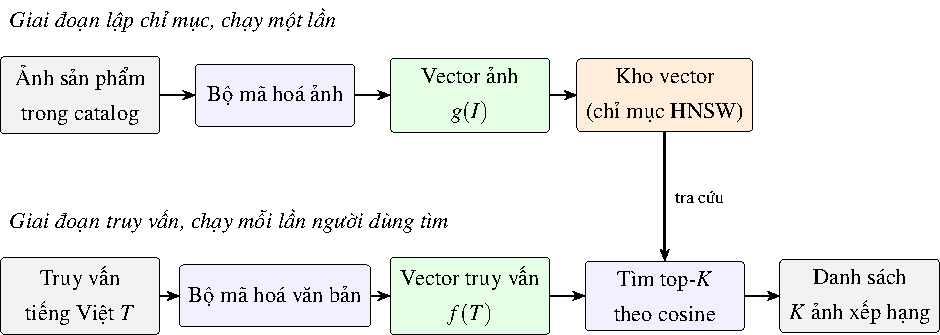
\includegraphics[width=0.96\textwidth]{graphics/fig_ch2_1.pdf}
\caption{Hai giai đoạn tìm kiếm dựa trên biểu diễn chung ảnh và văn bản}
\label{fig:ch2-pipeline}
\end{figure}

Hai không gian chỉ khớp nhau khi hai bộ mã hoá được huấn luyện chung, nên một bộ mã hoá văn bản tiếng Việt đơn mô thức không ghép trực tiếp được với bộ mã hoá ảnh của SigLIP~2. CLIP, SigLIP~2 và ViSigLIP-OT đều có sẵn cả bộ mã hoá ảnh lẫn bộ mã hoá văn bản: CLIP cho vector 512 chiều, SigLIP~2 và ViSigLIP-OT cho vector 768 chiều.
\subsection{Hàm mất mát tương phản}
\label{sec:ham-mat-mat}

Xét một lô gồm $B$ cặp ảnh--văn bản, với $x_i=g(I_i)$ và $y_i=f(T_i)$ là các vector đã chuẩn hoá. Logit của cặp $(i,j)$ là $z_{ij}=t\,x_i^{\top}y_j$, trong đó $t$ là hệ số tỷ lệ (nghịch đảo của nhiệt độ) được học cùng mô hình. CLIP coi cặp đúng $(i,i)$ là lớp đúng của một bài toán phân loại $B$ lớp và lấy entropy chéo theo cả hai chiều, từ ảnh sang văn bản và từ văn bản sang ảnh:
\begin{equation}
\mathcal{L}_{\mathrm{softmax}}=-\frac{1}{2B}\sum_{i=1}^{B}\left[\log\frac{e^{z_{ii}}}{\sum_{j=1}^{B}e^{z_{ij}}}+\log\frac{e^{z_{ii}}}{\sum_{j=1}^{B}e^{z_{ji}}}\right].
\label{eq:softmax}
\end{equation}
Mẫu số của mỗi số hạng cộng trên cả hàng hoặc cả cột, nên mọi phần tử khác trong lô đều là mẫu âm và chất lượng huấn luyện phụ thuộc cỡ lô $B$.

SigLIP bỏ phép chuẩn hoá này. Mỗi cặp $(i,j)$ là một bài toán phân loại nhị phân độc lập, với nhãn $\ell_{ij}=+1$ khi $i=j$ và $\ell_{ij}=-1$ trong các trường hợp còn lại; logit có thêm độ lệch $\beta$ học được, $z_{ij}=t\,x_i^{\top}y_j+\beta$. Bài báo gốc chia tổng cho $B$, còn đồ án chia cho $B^2$ (trung bình trên toàn bộ các cặp), nên giá trị mất mát nhỏ hơn $B$ lần:
\begin{equation}
\mathcal{L}_{\mathrm{sigmoid}}=-\frac{1}{B^{2}}\sum_{i=1}^{B}\sum_{j=1}^{B}\log\sigma\!\left(\ell_{ij}\,z_{ij}\right),\qquad \sigma(u)=\frac{1}{1+e^{-u}}.
\label{eq:sigmoid}
\end{equation}
Hình~\ref{fig:ch2-loss} đặt hai cách tính cạnh nhau trên ma trận độ tương đồng của một lô bốn cặp: ở CLIP, mỗi phép softmax phải nhìn thấy cả hàng (hoặc cả cột) tương ứng, còn ở SigLIP mỗi ô được chấm độc lập. Đồ án huấn luyện bằng hàm mất mát sigmoid theo cặp.

Mẫu âm khó của một sản phẩm là các sản phẩm gần nó nhất nhưng không phải cặp đúng; chúng làm bài toán phân biệt khó hơn so với mẫu âm ngẫu nhiên trong lô. Cách chọn mẫu âm khó của đồ án trình bày ở Mục~\ref{sec:tinh-chinh}.

\begin{figure}[H]
\centering
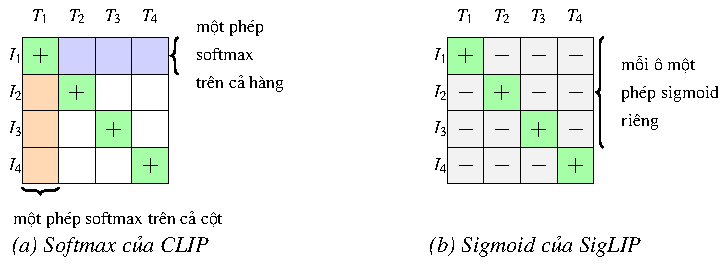
\includegraphics[width=0.9\textwidth]{graphics/fig_ch2_2.pdf}
\caption{So sánh hàm mất mát softmax và sigmoid trên ma trận độ tương đồng của một lô bốn cặp}
\label{fig:ch2-loss}
\end{figure}

\subsection{Tìm kiếm thưa BM25}
\label{sec:bm25}

BM25 chấm điểm một tài liệu $d$ cho truy vấn $q$ bằng cách cộng đóng góp của từng từ $w$ trong truy vấn:
\begin{equation}
\mathrm{BM25}(q,d)=\sum_{w\in q}\mathrm{IDF}(w)\cdot\frac{\mathrm{tf}(w,d)\,(k_1+1)}{\mathrm{tf}(w,d)+k_1\left(1-b+b\,\dfrac{|d|}{\mathrm{avgdl}}\right)},
\label{eq:bm25}
\end{equation}
trong đó $\mathrm{IDF}(w)=\ln\dfrac{N-n_w+0{,}5}{n_w+0{,}5}$, $\mathrm{tf}(w,d)$ là số lần từ $w$ xuất hiện trong $d$, $|d|$ là độ dài $d$, $\mathrm{avgdl}$ là độ dài trung bình của tài liệu, $N$ là số tài liệu và $n_w$ là số tài liệu chứa $w$. Tham số $k_1$ giới hạn mức tăng điểm theo tần suất từ, còn $b$ điều chỉnh mức phạt tài liệu dài. IDF của một từ có mặt trong hơn nửa số tài liệu sẽ âm; cài đặt của đồ án thay giá trị âm bằng một giá trị dương nhỏ, là $0{,}25$ lần IDF trung bình.

\subsection{Tìm kiếm vector gần đúng}
\label{sec:tim-kiem-gan-dung}

Với vector đã chuẩn hoá, xếp hạng theo cosine tương đương xếp hạng theo khoảng cách $L_2$. HNSW giảm chi phí này bằng đồ thị nhiều tầng: tầng trên cùng thưa, mỗi tầng dưới thêm nhiều nút hơn, và truy vấn đi tham lam từ tầng trên xuống để tới vùng chứa láng giềng gần nhất. Các tham số của đồ thị quyết định đánh đổi giữa tốc độ và tỷ lệ tìm đúng láng giềng thật.

\subsection{Tinh chỉnh hiệu quả tham số}
\label{sec:tinh-chinh-ly-thuyet}

Với ma trận trọng số gốc $W_0\in\mathbb{R}^{d_{\mathrm{out}}\times d_{\mathrm{in}}}$ được giữ cố định, LoRA học hai ma trận $U\in\mathbb{R}^{d_{\mathrm{out}}\times r}$ và $V\in\mathbb{R}^{r\times d_{\mathrm{in}}}$ với hạng $r\ll\min(d_{\mathrm{out}},d_{\mathrm{in}})$ và cộng tích của chúng vào trọng số gốc:
\begin{equation}
W=W_0+\frac{\alpha}{r}\,UV.
\label{eq:lora}
\end{equation}
DoRA tách trọng số thành độ lớn $m$ (vector học được) và hướng, rồi chỉ dùng phần cập nhật hạng thấp để điều chỉnh hướng. Với $W'=W_0+\frac{\alpha}{r}UV$, vector $m\in\mathbb{R}^{d_{\mathrm{out}}}$ có một phần tử cho mỗi đầu ra, và $\lVert W'\rVert_{\mathrm{row}}\in\mathbb{R}^{d_{\mathrm{out}}}$ là chuẩn $L_2$ của từng hàng $W'$ (mỗi hàng ứng với một đầu ra):
\begin{equation}
W=\mathrm{diag}(m)\,\mathrm{diag}\bigl(\lVert W'\rVert_{\mathrm{row}}\bigr)^{-1}W'.
\label{eq:dora}
\end{equation}

\subsection{Chỉ số đánh giá}
\label{sec:chi-so-danh-gia}

Mỗi cặp truy vấn--sản phẩm do người chấm xem được ít nhất hai người chấm độc lập theo thang 0 (không liên quan), 1 (liên quan một phần) và 2 (liên quan chính xác). Điểm của cặp là trung bình các điểm đó, nên có thể nhận giá trị lẻ như 0,5 hoặc 1,5; cặp được tính là liên quan khi điểm trung bình từ 1 trở lên. Cặp xuất hiện trong $K$ kết quả đầu mà chưa có nhãn được tính là không liên quan. Độ đồng thuận giữa các người chấm đo bằng hệ số kappa của Cohen~\cite{cohen1960kappa} và diễn giải theo thang của Landis và Koch~\cite{landis1977kappa}.

Gọi $Q$ là tập truy vấn, $D^{q}_i$ là kết quả hạng $i$ của truy vấn $q$ và $\mathbb{1}_{\mathrm{rel}}(q,D)$ cho biết cặp liên quan hay không. Recall@$K$ trong đồ án là tỷ lệ truy vấn có ít nhất một kết quả liên quan trong $K$ kết quả đầu. Đây là tỷ lệ trúng, khác với cách BEIR~\cite{thakur2021beir} tính Recall theo tỷ lệ tài liệu liên quan tìm lại được, nên số liệu hai bên không đặt cạnh nhau được:
\begin{equation}
\mathrm{Recall@}K=\frac{1}{|Q|}\sum_{q\in Q}\mathbb{1}\Bigl[\exists\, i\le K:\ \mathbb{1}_{\mathrm{rel}}\bigl(q,D^{q}_i\bigr)\Bigr].
\label{eq:recall}
\end{equation}
MRR lấy trung bình nghịch đảo hạng của kết quả liên quan đầu tiên, $r_q$; số hạng của truy vấn không có kết quả liên quan trong danh sách bằng 0:
\begin{equation}
\mathrm{MRR}=\frac{1}{|Q|}\sum_{q\in Q}\frac{1}{r_q}.
\label{eq:mrr}
\end{equation}
nDCG@$K$ dùng điểm liên quan $\mathrm{rel}_i$ của kết quả hạng $i$. Mỗi kết quả đóng góp $2^{\mathrm{rel}_i}-1$ điểm, giảm dần theo logarit của hạng; IDCG là DCG của thứ tự lý tưởng, tính trên các cặp đã có nhãn của cùng truy vấn:
\begin{equation}
\mathrm{nDCG@}K=\frac{\mathrm{DCG@}K}{\mathrm{IDCG@}K},\qquad \mathrm{DCG@}K=\sum_{i=1}^{K}\frac{2^{\mathrm{rel}_i}-1}{\log_2(i+1)}.
\label{eq:ndcg}
\end{equation}
Đồ án loại khỏi trung bình nDCG những truy vấn không có cặp nào đạt điểm liên quan từ 1 trở lên, vì IDCG của chúng bằng 0. Recall và MRR vẫn giữ các truy vấn này với giá trị 0, nên mẫu số của ba chỉ số không giống nhau.

Để so sánh hai hệ $S_1$ và $S_2$ trên cùng tập truy vấn, đồ án dùng kiểm định bootstrap ghép cặp theo truy vấn. Gọi $\Delta$ là hiệu trung bình của chỉ số theo từng truy vấn giữa $S_1$ và $S_2$. Phép kiểm định lấy mẫu lại các truy vấn có hoàn lại $R$ lần, tính $\Delta^{*}_r$ trên mỗi lần lấy mẫu, và khi $\Delta>0$ thì giá trị $p$ hai phía là
\begin{equation}
p=\frac{2}{R}\sum_{r=1}^{R}\mathbb{1}\bigl[\Delta^{*}_r\le 0\bigr],
\label{eq:bootstrap}
\end{equation}
với dấu bất đẳng thức đổi chiều khi $\Delta<0$, và $p$ được giới hạn ở 1. Đồ án không hiệu chỉnh các giá trị $p$ cho nhiều phép so sánh.

\chapter{Phân tích và thiết kế hệ thống}
\label{chap:thiet_ke}

Chương này trình bày yêu cầu, chức năng, kiến trúc, các luồng xử lý, các thành phần, mô hình dữ liệu và giao diện của hệ thống.

\section{Yêu cầu của hệ thống}
\label{sec:yeu-cau}

\subsection{Đối tượng sử dụng}

Hệ thống phục vụ ba nhóm đối tượng. \textbf{Người dùng cuối} mô tả món đồ bằng tiếng Việt hoặc tải một ảnh mẫu lên, rồi nhận danh sách sản phẩm gần nhất trong catalog qua giao diện web. \textbf{Developer} là các thành viên của nhóm; họ lập chỉ mục catalog, chạy đánh giá, kiểm định thống kê và tinh chỉnh mô hình (FR05 đến FR08). \textbf{Người gán nhãn} chấm điểm liên quan 0, 1 hoặc 2 cho từng cặp truy vấn--sản phẩm (FR09). Hệ thống không có tài khoản; dịch vụ chạy cục bộ, có thể bảo vệ bằng một khoá API dùng chung.

\subsection{Yêu cầu chức năng}

Bảng~\ref{tab:c3_fr} liệt kê chín yêu cầu chức năng; bốn yêu cầu đầu dành cho người dùng cuối, năm yêu cầu sau phục vụ việc xây dựng và so sánh các hệ tìm kiếm.

\begin{table}[!htbp]
\centering
\caption{Yêu cầu chức năng}
\label{tab:c3_fr}
\footnotesize
\renewcommand{\arraystretch}{1.0}
\begin{tabularx}{\textwidth}{@{}p{1.2cm} >{\raggedright\arraybackslash}X p{2.6cm}@{}}
\toprule
\textbf{Mã} & \textbf{Yêu cầu} & \textbf{Tác nhân} \\
\midrule
FR01 & Tìm sản phẩm bằng mô tả tiếng Việt dài từ 1 đến 512 ký tự; trả về $K$ kết quả ($K$ từ 1 đến 100), xếp hạng và kèm điểm tương đồng & Người dùng cuối \\
FR02 & Tìm sản phẩm bằng ảnh tải lên, tối đa 8 MiB; chỉ áp dụng khi cấu hình dùng bộ tìm kiếm vector, vì BM25 từ chối truy vấn chỉ có ảnh & Người dùng cuối \\
FR03 & Lọc kết quả theo một danh mục, cho cả tìm bằng chữ và tìm bằng ảnh & Người dùng cuối \\
FR04 & Hiển thị trạng thái hệ thống: tên bộ tìm kiếm, số sản phẩm đã lập chỉ mục, và trạng thái suy giảm khi kho vector không trả lời & Người dùng cuối \\
FR05 & Lập chỉ mục catalog bằng mô hình đã đăng ký: mã hoá ảnh sản phẩm và ghi vào kho theo từng lô; có tuỳ chọn xoá rồi tạo lại bộ sưu tập (collection, nhóm vector cùng chiều trong kho) & Developer \\
FR06 & Chạy một hệ tìm kiếm trên bộ truy vấn, lưu 20 kết quả đầu, tính Recall@1/5/10, MRR, nDCG@10 và ghi nhật ký thí nghiệm & Developer \\
FR07 & Kiểm định chênh lệch giữa hai hệ bằng bootstrap ghép cặp theo truy vấn (lấy mẫu lại các truy vấn); tính hệ số kappa giữa những người chấm & Developer \\
FR08 & Tinh chỉnh SigLIP~2 bằng LoRA hoặc DoRA; dùng GradCache (tích luỹ gradient theo từng khối nhỏ) để huấn luyện với kích thước lô lớn; lưu lại bản trọng số có Recall@5 cao nhất trên tập xác thực & Developer \\
FR09 & Gán nhãn mù 0/1/2 cho cặp truy vấn--sản phẩm, ghi riêng theo từng người chấm, cho phép hoàn tác điểm vừa chấm & Người gán nhãn \\
\bottomrule
\end{tabularx}
\end{table}

\subsection{Yêu cầu phi chức năng}

Bảng~\ref{tab:c3_nfr} nêu các yêu cầu phi chức năng cùng chỉ tiêu. NFR04 và NFR02 chi phối kiến trúc nhiều nhất. NFR04 buộc mọi hệ được đo trong cùng điều kiện, nếu không bảng xếp hạng không có giá trị so sánh; NFR02 buộc hệ thống chạy được trên máy cá nhân để người khác tái lập đồ án.

\begin{table}[!htbp]
\centering
\caption{Yêu cầu phi chức năng và chỉ tiêu}
\label{tab:c3_nfr}
\footnotesize
\renewcommand{\arraystretch}{1.0}
\begin{tabularx}{\textwidth}{@{}p{1.3cm} p{2.3cm} >{\raggedright\arraybackslash}X >{\raggedright\arraybackslash}X@{}}
\toprule
\textbf{Mã} & \textbf{Thuộc tính} & \textbf{Yêu cầu} & \textbf{Chỉ tiêu} \\
\midrule
NFR01 & Độ trễ & Một truy vấn chữ trả kết quả đủ nhanh để dùng tương tác & p95 của thời gian mã hoá và tìm dưới 200 ms trên máy phát triển, với kho trong bộ nhớ. Đề cương không nêu phân vị nên đồ án chọn p95 \\
NFR02 & Chạy nhẹ & Lõi, API web và bộ kiểm thử chạy được với các gói nhẹ, không cần GPU, Qdrant hay tải mô hình & Khởi động bằng cấu hình mặc định; bộ kiểm thử mặc định chạy không lỗi \\
NFR03 & Khả năng thay thế & Thêm một mô hình hoặc một kho vector mới không phải sửa lõi & Mọi bộ mã hoá và kho vector đi qua cùng một bộ tìm kiếm vector của lõi; thêm bộ chuyển đổi mới chỉ cần thêm một tệp và khai báo trong bộ đăng ký \\
NFR04 & So sánh được & Mọi hệ dùng chung cổng tìm kiếm, bộ truy vấn và định nghĩa chỉ số & Các hệ dùng chung một tệp truy vấn và một tệp nhãn \\
NFR05 & Tái lập & Cấu hình tập trung; mỗi lần chạy được ghi lại & Giá trị khởi tạo ngẫu nhiên cố định; mỗi lần đánh giá hoặc huấn luyện thêm một dòng vào nhật ký 16 cột \\
NFR06 & Bảo mật đầu vào & Khoá API tuỳ chọn; giới hạn kích thước đầu vào & Khi đặt khoá, khoá sai bị từ chối (401); ảnh quá 8 MiB bị từ chối (413), ảnh rỗng (422) \\
NFR07 & Chịu lỗi kho vector & Mất kết nối kho không làm sập API web & Trạng thái hệ thống báo suy giảm; tìm kiếm trả 503 với thông báo cố định, không lộ địa chỉ kho \\
NFR08 & Quy mô catalog & Phục vụ catalog có quy mô như đề cương nêu & 20.000 đến 50.000 sản phẩm \\
\bottomrule
\end{tabularx}
\end{table}

Mức đạt của từng yêu cầu được đối chiếu ở Mục~\ref{sec:ke-hoach-kiem-thu} của Chương~\ref{chap:danh_gia}. Hai yêu cầu chưa đạt là NFR08, do catalog thực tế chỉ có 6.963 ảnh, và NFR01 với hệ DoRA; số đo của NFR01 nằm ở Chương~\ref{chap:danh_gia}.

\section{Chức năng và kịch bản sử dụng}
\label{sec:chuc-nang}

Hình~\ref{fig:c3_chucnang} nối chín chức năng với ba tác nhân. Người dùng cuối dùng FR01 đến FR04 qua giao diện web; Developer và người gán nhãn dùng các công cụ dòng lệnh và một máy chủ gán nhãn nhỏ chạy cục bộ. Trong chín chức năng, lọc theo danh mục (FR03) và kiểm định thống kê (FR07) là tuỳ chọn; bảy chức năng còn lại cần có để hệ thống tìm kiếm và đánh giá hoạt động. Bảng~\ref{tab:c3_uc01} và Bảng~\ref{tab:c3_uc02} mô tả hai kịch bản của người dùng cuối; luồng lập chỉ mục của Developer nằm ở Mục~\ref{sec:luong-xu-ly}.

\begin{figure}[!htbp]
\centering
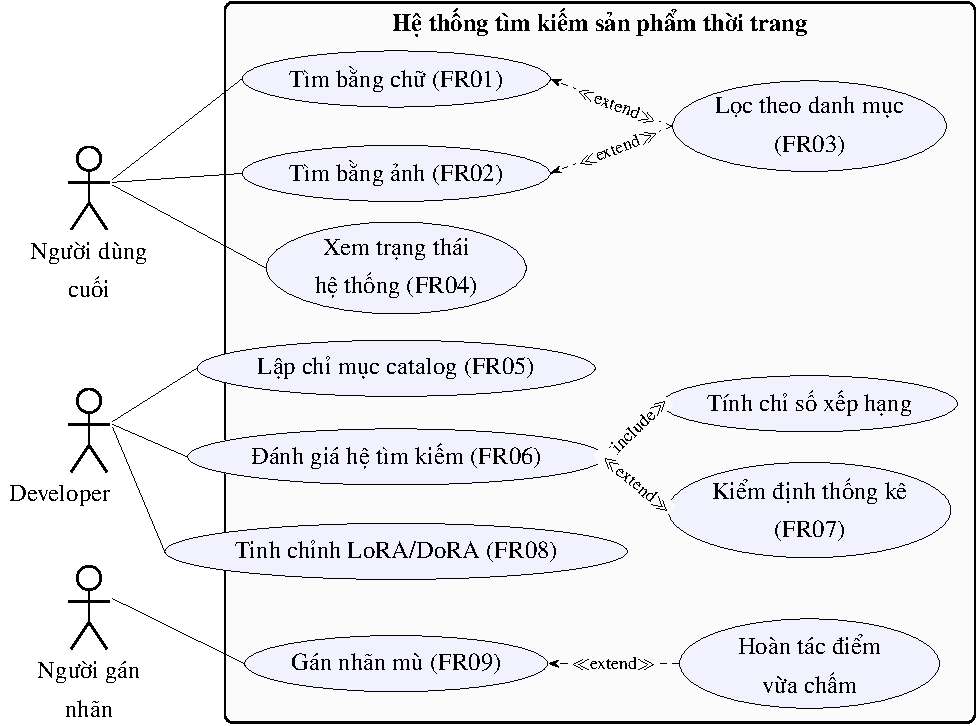
\includegraphics[width=0.9\textwidth]{graphics/fig_ch3_1.pdf}
\caption{Sơ đồ chức năng theo ba nhóm tác nhân}
\label{fig:c3_chucnang}
\end{figure}

\begin{table}[!htbp]
\centering
\caption{Kịch bản UC01, tìm sản phẩm bằng mô tả chữ}
\label{tab:c3_uc01}
\footnotesize
\renewcommand{\arraystretch}{1.05}
\begin{tabularx}{\textwidth}{@{}p{3.0cm} >{\raggedright\arraybackslash}X@{}}
\toprule
\textbf{Chức năng} & Tìm sản phẩm bằng mô tả chữ (FR01, FR03) \\
\midrule
\textbf{Tác nhân} & Người dùng cuối \\
\midrule
\textbf{Điều kiện ban đầu} & API web đang chạy với một bộ tìm kiếm đã cấu hình; catalog đã được lập chỉ mục \\
\midrule
\textbf{Luồng chính} & 1. Người dùng nhập mô tả, chẳng hạn ``áo len dệt kim xám'', rồi nhấn nút Tìm.\newline
2. Giao diện gửi mô tả cùng số kết quả mong muốn tới API web.\newline
3. API web kiểm tra khoá (nếu máy chủ bật khoá) và độ dài mô tả.\newline
4. Bộ tìm kiếm mã hoá câu và lấy từ kho các vector gần nhất.\newline
5. Giao diện hiển thị lưới thẻ kết quả theo hạng, mỗi thẻ có ảnh, tiêu đề, danh mục và độ tương đồng \\
\midrule
\textbf{Luồng rẽ nhánh} & 1a. Người dùng chọn một danh mục: yêu cầu mang thêm bộ lọc theo tên danh mục.\newline
1b. Người dùng đã chọn một ảnh trước đó: nút Tìm chạy kịch bản UC02 thay cho kịch bản này \\
\midrule
\textbf{Ngoại lệ} & Bước 1: ô mô tả trống và chưa chọn ảnh, giao diện nhắc nhập mô tả và không gửi yêu cầu.\newline
Bước 3: khoá API sai, API web trả 401.\newline
Bước 4: kho vector không phản hồi, API web trả 503.\newline
Bước 5: không có sản phẩm nào khớp bộ lọc, giao diện gợi ý đổi mô tả hoặc bỏ bộ lọc \\
\midrule
\textbf{Kết quả} & Người dùng nhận tối đa $K$ sản phẩm xếp theo độ gần với mô tả \\
\bottomrule
\end{tabularx}
\end{table}

\begin{table}[!htbp]
\centering
\caption{Kịch bản UC02, tìm sản phẩm bằng ảnh}
\label{tab:c3_uc02}
\footnotesize
\renewcommand{\arraystretch}{1.05}
\begin{tabularx}{\textwidth}{@{}p{3.0cm} >{\raggedright\arraybackslash}X@{}}
\toprule
\textbf{Chức năng} & Tìm sản phẩm bằng ảnh mẫu (FR02, FR03) \\
\midrule
\textbf{Tác nhân} & Người dùng cuối \\
\midrule
\textbf{Điều kiện ban đầu} & Như UC01, và bộ tìm kiếm của cấu hình là loại vector; BM25 không mã hoá được ảnh \\
\midrule
\textbf{Luồng chính} & 1. Người dùng kéo ảnh vào vùng thả hoặc chọn tệp jpg, jpeg, png hay webp, rồi nhấn nút Tìm.\newline
2. Giao diện gửi ảnh cùng số kết quả mong muốn tới API web.\newline
3. API web kiểm tra khoá, ảnh không rỗng và dung lượng không quá 8 MiB.\newline
4. Bộ tìm kiếm mã hoá ảnh bằng chính bộ mã hoá đã lập chỉ mục catalog và lấy từ kho các vector gần nhất.\newline
5. Giao diện hiển thị lưới thẻ kết quả như ở UC01 \\
\midrule
\textbf{Luồng rẽ nhánh} & 1a. Người dùng bấm nút bỏ ảnh: giao diện quay về tìm bằng chữ.\newline
2a. Người dùng đã chọn danh mục: yêu cầu mang thêm trường danh mục \\
\midrule
\textbf{Ngoại lệ} & Bước 1: ảnh lớn hơn 8 MiB, giao diện từ chối ngay và không gửi.\newline
Bước 3: ảnh rỗng, API web trả 422; ảnh quá lớn mà vẫn tới được máy chủ, API web trả 413.\newline
Bước 4: cấu hình dùng BM25, API web trả 501; kho vector không phản hồi, API web trả 503 \\
\midrule
\textbf{Kết quả} & Người dùng nhận tối đa $K$ sản phẩm có vector gần vector của ảnh mẫu \\
\bottomrule
\end{tabularx}
\end{table}

\section{Kiến trúc hệ thống}
\label{sec:kien-truc}

\subsection{Các tầng của hệ thống}

Hình~\ref{fig:c3_kientruc} mô tả hệ thống theo mô hình cổng và bộ chuyển đổi~\cite{cockburn2005hexagonal}, gồm bốn tầng. Cổng là giao diện trừu tượng do lõi định nghĩa; bộ chuyển đổi là phần cài đặt cụ thể của một cổng.

\begin{itemize}
\setlength{\itemsep}{1pt}
\item Tầng 1 là các điểm vào: giao diện web cùng API web, công cụ lập chỉ mục, công cụ đánh giá (kể cả thí nghiệm loại bỏ từng thành phần), công cụ huấn luyện và công cụ gán nhãn.
\item Tầng 2 là lõi, gồm các thực thể của mô hình miền, các cổng và bộ tìm kiếm vector. Lõi chỉ dùng thư viện chuẩn nên chạy được khi chưa cài thư viện học máy nào.
\item Tầng 3 gồm các bộ chuyển đổi cài đặt cổng của lõi: mô hình nhúng, kho vector, bộ tìm kiếm từ khoá BM25 và bộ chỉ số. Phần huấn luyện và các phép kiểm định thống kê cũng thuộc tầng này nhưng không cài đặt cổng nào. Huấn luyện chỉ dùng thực thể sản phẩm; kiểm định là hàm bổ sung của bộ chỉ số.
\item Tầng 4 là tài nguyên bên ngoài: trọng số mô hình, trọng số bổ sung của LoRA, Qdrant, tệp catalog, ảnh, truy vấn, nhãn và nhật ký thí nghiệm.
\end{itemize}

\begin{figure}[!htbp]
\centering
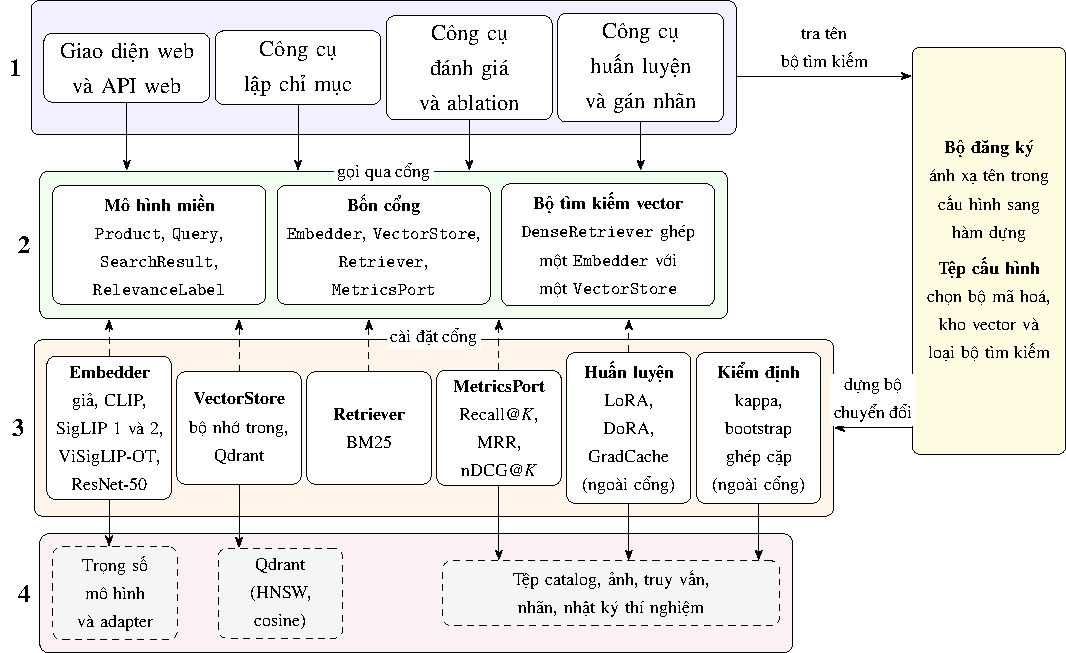
\includegraphics[width=\textwidth]{graphics/fig_ch3_2.pdf}
\caption{Kiến trúc bốn tầng theo mô hình cổng và bộ chuyển đổi}
\label{fig:c3_kientruc}
\end{figure}

Phụ thuộc đi một chiều: tầng 1 gọi lõi qua cổng, bộ chuyển đổi ở tầng 3 phụ thuộc vào cổng của lõi, còn lõi không biết bộ chuyển đổi nào tồn tại. Bộ đăng ký đọc tên trong tệp cấu hình và dựng bộ chuyển đổi tương ứng.

\subsection{Các lựa chọn thiết kế chính}

\begin{enumerate}
\setlength{\itemsep}{2pt}
\item \textbf{Bốn cổng ở lõi.} Lõi định nghĩa bốn cổng cho bộ mã hoá, kho vector, bộ tìm kiếm và bộ chỉ số. Mỗi mô hình, kho vector hay cách tìm kiếm là một bộ chuyển đổi cài đặt một cổng; nhờ vậy các hệ được so sánh trong chương đánh giá dùng chung một quy trình đánh giá (NFR03, NFR04).
\item \textbf{Cấu hình chọn bộ chuyển đổi.} Tệp cấu hình ghi tên bộ mã hoá, kho vector và loại bộ tìm kiếm; bộ đăng ký chỉ nạp các bộ chuyển đổi nặng khi được gọi tên. Cấu hình mặc định dùng bộ mã hoá mô phỏng 64 chiều và kho trong bộ nhớ, nên hệ thống khởi động được mà không cần GPU hay Qdrant (NFR02).
\item \textbf{Catalog được lập chỉ mục bằng ảnh.} Catalog chỉ có tên danh mục, không có mô tả màu hay chất liệu, nên vector của sản phẩm lấy từ ảnh. Công cụ lập chỉ mục gọi thẳng bộ mã hoá ảnh rồi ghi vector vào kho. Tài liệu của BM25 vì thế chỉ gồm tên danh mục tiếng Việt; Chương~\ref{chap:danh_gia} bàn hệ quả của điều này với việc so sánh các hệ.
\item \textbf{Hai kho vector cho hai mục đích.} Kho trong bộ nhớ tìm chính xác và được dùng để đánh giá, đo độ trễ; Qdrant tìm gần đúng bằng HNSW~\cite{malkov2020hnsw} và được dùng cho trình diễn. Các chỉ số đánh giá nhờ vậy không chịu ảnh hưởng của phép tìm gần đúng; mức chênh giữa hai kho nằm ở Mục~\ref{sec:han-che-danh-gia}.
\item \textbf{Truy vấn chữ và truy vấn ảnh xử lý riêng.} API web nhận truy vấn chữ hoặc truy vấn ảnh, không nhận cả hai cùng lúc, vì đồ án không hợp nhất vector chữ và vector ảnh. Truy vấn ảnh đi qua bộ mã hoá ảnh của chính mô hình SigLIP~2 đã tinh chỉnh đang phục vụ tìm bằng chữ, nên ảnh truy vấn và ảnh catalog nằm trong cùng không gian vector. Đồ án đánh giá truy vấn bằng chữ (Mục~\ref{sec:han-che-danh-gia}).
\end{enumerate}

\section{Các luồng xử lý chính}
\label{sec:luong-xu-ly}

\subsection{Lập chỉ mục catalog}

Luồng lập chỉ mục (Hình~\ref{fig:c3_hoatdong}) bắt đầu bằng việc đọc cấu hình và danh sách sản phẩm, rồi dựng bộ mã hoá và kho qua bộ đăng ký. Chế độ mã hoá bằng ảnh chỉ chạy với bộ tìm kiếm vector; nếu cấu hình dùng loại khác, công cụ dừng trước khi xoá hay ghi bất cứ dữ liệu nào. Tiếp theo, bộ sưu tập được tạo nếu chưa có, hoặc xoá rồi tạo lại khi người dùng yêu cầu. Với mỗi lô, công cụ mã hoá ảnh thành vector chuẩn hoá $L_2$ và ghi vào kho kèm thuộc tính sản phẩm. Chạy lại cùng catalog thì sản phẩm cũ bị ghi đè chứ không nhân đôi. Khi gặp ảnh không đọc được, công cụ dừng, báo mã sản phẩm và giữ nguyên các lô đã ghi.

\begin{figure}[!htbp]
\centering
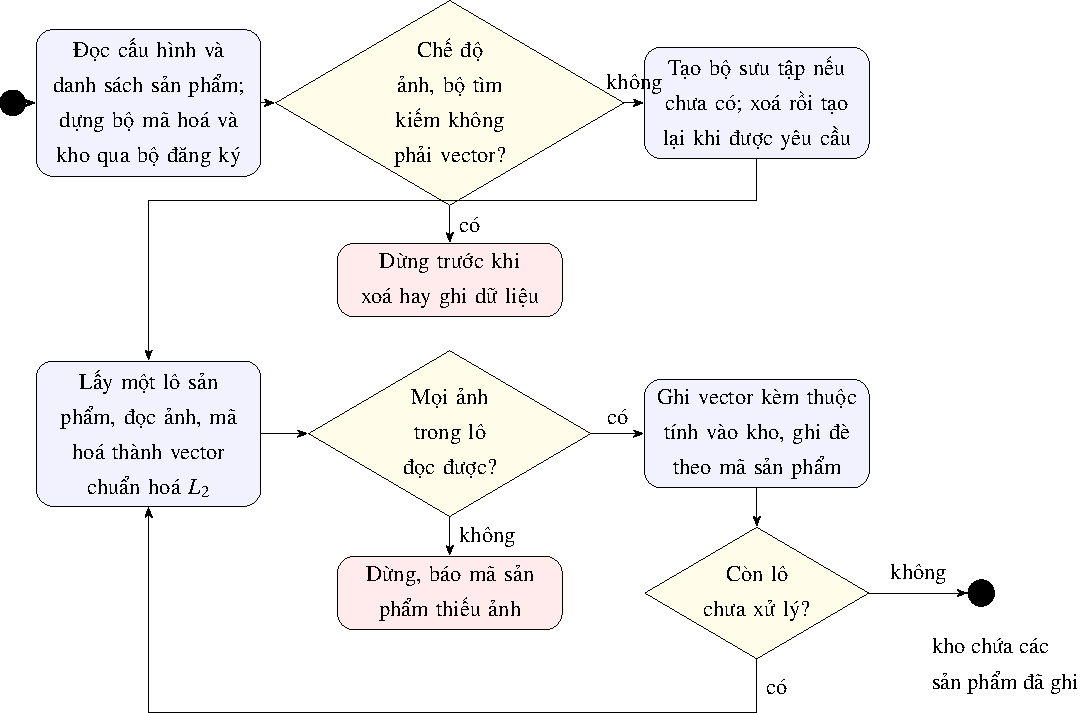
\includegraphics[width=0.85\textwidth]{graphics/fig_ch3_3.pdf}
\caption{Biểu đồ hoạt động của luồng lập chỉ mục catalog}
\label{fig:c3_hoatdong}
\end{figure}

\subsection{Tìm kiếm bằng chữ}

Hình~\ref{fig:c3_tuantu} là biểu đồ tuần tự của một truy vấn chữ. API web kiểm tra đầu vào rồi tạo một đối tượng truy vấn với mã ngẫu nhiên, số kết quả và bộ lọc. Bộ tìm kiếm vector chuẩn hoá câu về dạng NFC và chữ thường, rồi gọi bộ mã hoá để đổi câu thành vector chuẩn hoá $L_2$. Sau đó nó lấy từ kho $K$ sản phẩm gần nhất theo độ tương đồng cosine, kèm bộ lọc danh mục nếu có. Các trường hợp lỗi nằm ở Bảng~\ref{tab:c3_uc01}. Luồng tìm bằng ảnh chỉ khác ở bước mã hoá. Với BM25, bộ tìm kiếm tự chấm điểm theo từ, không qua bộ mã hoá và kho.

\begin{figure}[!htbp]
\centering
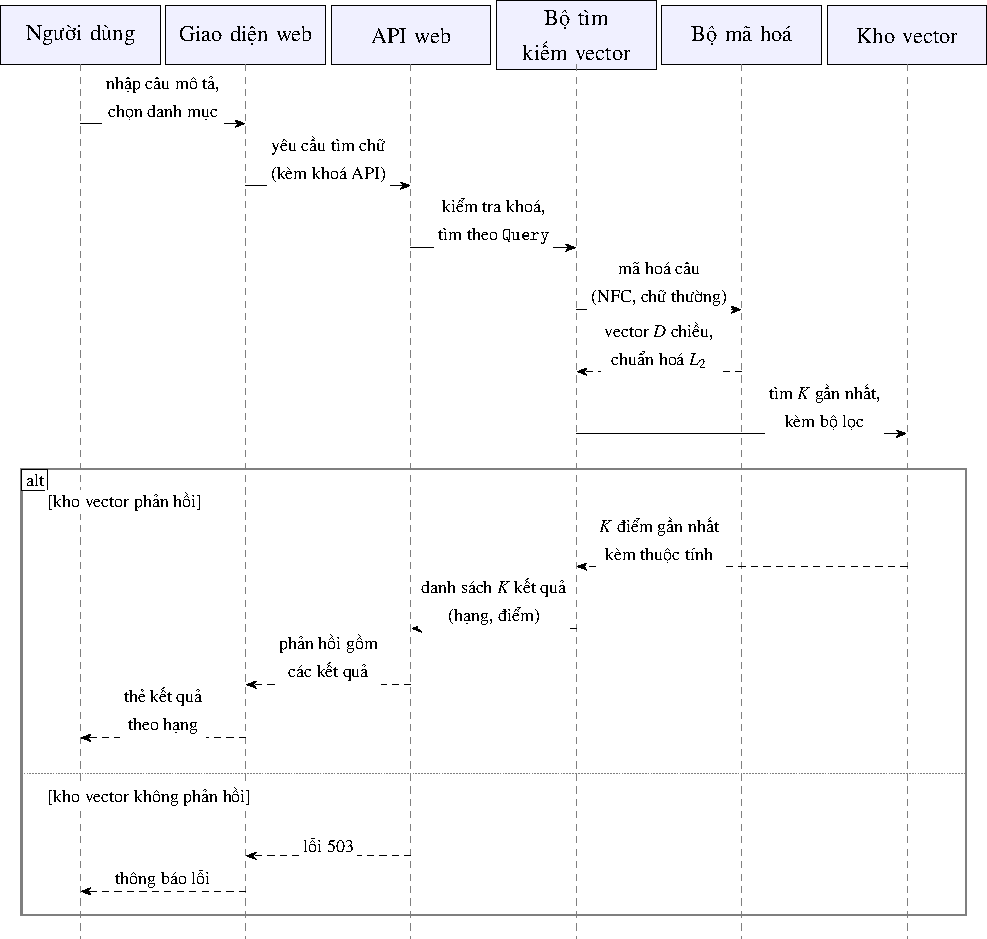
\includegraphics[width=0.88\textwidth]{graphics/fig_ch3_4.pdf}
\caption{Biểu đồ tuần tự của luồng tìm kiếm bằng chữ}
\label{fig:c3_tuantu}
\end{figure}

\section{Các thành phần chính}
\label{sec:thanh-phan}

Hình~\ref{fig:c3_lop} vẽ bốn cổng, bộ tìm kiếm vector của lõi (tô xanh) và các bộ chuyển đổi. Hệ thống có bốn bộ mã hoá dùng trong đánh giá: bộ mô phỏng 64 chiều, CLIP 512 chiều, SigLIP~2 768 chiều và ViSigLIP-OT 768 chiều; kèm hai kho vector, bộ tìm kiếm BM25 và bộ tính chỉ số xếp hạng.

Bộ mã hoá SigLIP~2 cũng nạp được SigLIP~1 khi đổi tên bản trọng số; danh sách mô hình cụ thể nằm ở Bảng~\ref{tab:c4_mahoa}. Bộ tìm kiếm vector thuộc lõi: nó ghép một bộ mã hoá với một kho vector để cài đặt cổng tìm kiếm, nên mọi cặp bộ mã hoá và kho đều dùng chung bộ này. BM25 cài đặt cùng cổng nhưng giữ chỉ mục riêng và không dùng kho.


\begin{figure}[!htbp]
\centering
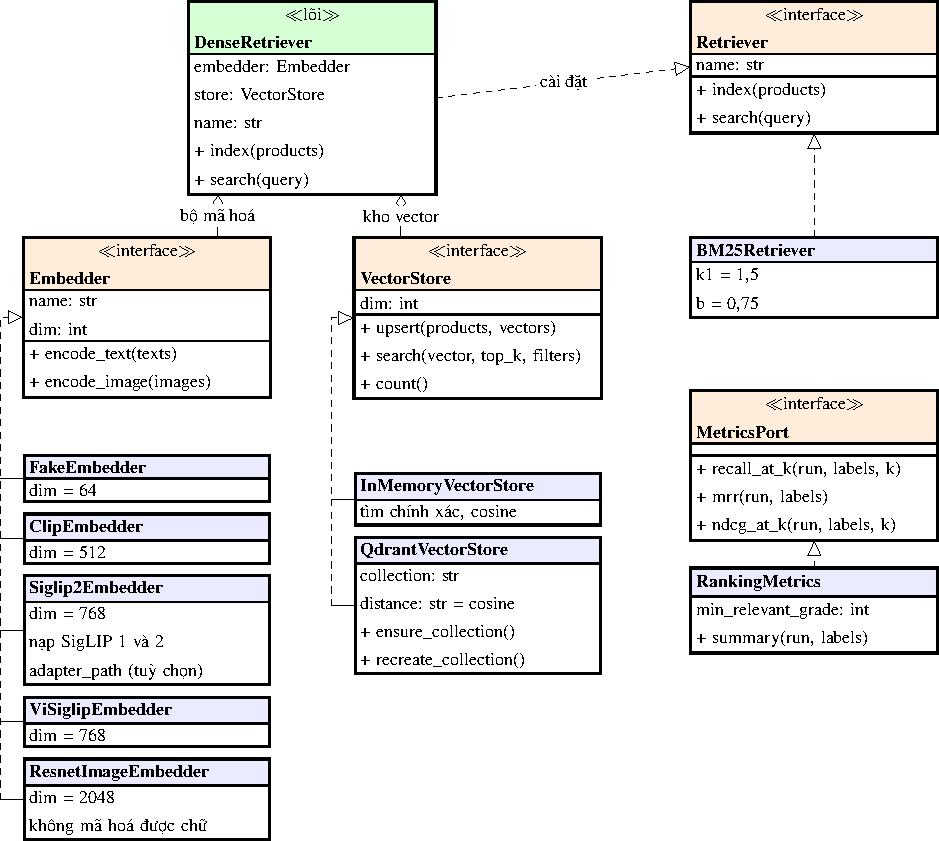
\includegraphics[width=0.86\textwidth]{graphics/fig_ch3_5.pdf}
\caption{Biểu đồ lớp của các cổng và bộ chuyển đổi}
\label{fig:c3_lop}
\end{figure}

\section{Cơ sở dữ liệu}
\label{sec:co-so-du-lieu}

\subsection{Các thực thể và quan hệ}

Hệ thống không dùng cơ sở dữ liệu quan hệ; dữ liệu nằm ở các tệp văn bản và ở kho vector (Hình~\ref{fig:c3_erd}). Một truy vấn của bộ đánh giá có nhiều kết quả và nhiều nhãn; một sản phẩm xuất hiện trong nhiều kết quả và nhiều nhãn; mỗi sản phẩm có một vector trong mỗi bộ sưu tập của kho vector. Khi đánh giá, hệ thống ghi 20 kết quả đầu của từng hệ kèm mã truy vấn và tên hệ. Các bản ghi này hợp thành tập cặp cần chấm, tức các cặp truy vấn--sản phẩm chờ gán nhãn.

\begin{figure}[!htbp]
\centering
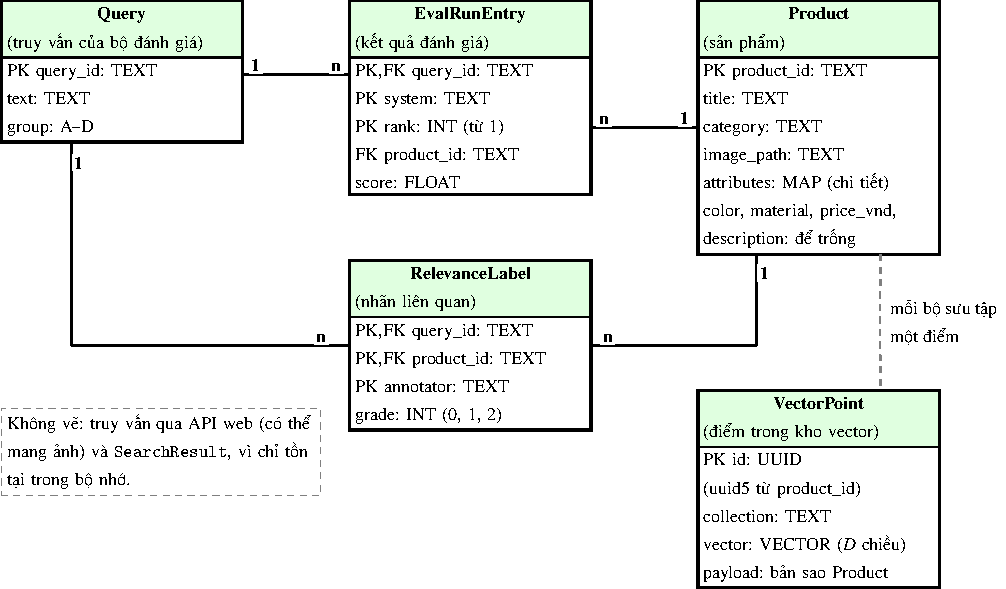
\includegraphics[width=0.88\textwidth]{graphics/fig_ch3_6.pdf}
\caption{Mô hình dữ liệu logic của hệ thống}
\label{fig:c3_erd}
\end{figure}

\subsection{Mô tả các bảng}

Bảng~\ref{tab:c3_thucthe} mô tả các thực thể. Về nơi lưu, catalog đã chuẩn bị, bộ 155 truy vấn và tập cặp cần chấm là các tệp JSON; nhãn của người chấm là các tệp JSONL, mỗi người một tệp, chỉ ghi nối thêm; nhật ký thí nghiệm là một tệp CSV 16 cột; vector sản phẩm nằm trong bộ sưu tập của kho.

Mỗi sản phẩm trong catalog chỉ có tên, danh mục, đường dẫn ảnh và chi tiết bộ phận trong trường thuộc tính. Màu, chất liệu, giá và mô tả để trống vì nguồn dữ liệu không có. Nhãn tự động do bộ lọc chấm 0 tạo ra (Mục~\ref{sec:du-lieu-cach-do}) luôn có điểm 0 và mang tên \texttt{auto-filter} ở cột người chấm. Bộ chỉ số coi cặp nằm trong $K$ kết quả đầu mà chưa có nhãn là không liên quan, đồng thời báo số cặp thiếu nhãn. Do đó Recall@10 là cận dưới của giá trị thật (Chương~\ref{chap:danh_gia}).

\begin{table}[!htbp]
\centering
\caption{Các thực thể của mô hình dữ liệu}
\label{tab:c3_thucthe}
\footnotesize
\renewcommand{\arraystretch}{1.05}
\begin{tabularx}{\textwidth}{@{}p{3.1cm} >{\raggedright\arraybackslash}X >{\raggedright\arraybackslash}X@{}}
\toprule
\textbf{Thực thể} & \textbf{Trường chính} & \textbf{Ràng buộc} \\
\midrule
\texttt{Product} & \texttt{product\_id}, \texttt{title}, \texttt{category}, \texttt{image\_path}, \texttt{attributes}, và bốn trường tuỳ chọn \texttt{color}, \texttt{material}, \texttt{price\_vnd}, \texttt{description} & Mã và tiêu đề không rỗng; giá không âm \\
\texttt{Query} & \texttt{query\_id}, \texttt{text}, \texttt{image\_bytes}, \texttt{image\_path}, \texttt{top\_k}, \texttt{filters}; ở bộ đánh giá có thêm \texttt{group} (nhóm A đến D) & Mã truy vấn không rỗng; có chữ hoặc ảnh; \texttt{top\_k} $\geq 1$ \\
\texttt{SearchResult} & \texttt{product}, \texttt{score}, \texttt{rank} & Hạng đánh số từ 1; chỉ có trong bộ nhớ, không lưu \\
\texttt{EvalRunEntry} & \texttt{query\_id}, \texttt{system}, \texttt{rank}, \texttt{product\_id}, \texttt{score} & Khoá là (\texttt{query\_id}, \texttt{system}, \texttt{rank}); mỗi hệ giữ 20 kết quả đầu \\
\texttt{RelevanceLabel} & \texttt{query\_id}, \texttt{product\_id}, \texttt{grade}, \texttt{annotator} (tên người chấm, hoặc \texttt{auto-filter} với nhãn tự động) & Điểm thuộc $\{0, 1, 2\}$ \\
\texttt{VectorPoint} & mã bản ghi trong kho, vector $D$ chiều ($D$ do bộ mã hoá quyết định), bản sao thuộc tính sản phẩm & Ở Qdrant, mã là \texttt{uuid5} của \texttt{product\_id}; kho trong bộ nhớ khoá thẳng theo \texttt{product\_id}; mỗi bản trọng số có một bộ sưu tập \\
\bottomrule
\end{tabularx}
\end{table}

\section{Giao diện người dùng}
\label{sec:giao-dien}

Giao diện web là một màn hình duy nhất, không chuyển trang (Hình~\ref{fig:c3_dieuhuong}): thanh trên hiện trạng thái hệ thống, hai phần tìm bằng chữ và bằng ảnh cùng hiển thị kết quả trên một lưới.

\begin{figure}[!htbp]
\centering
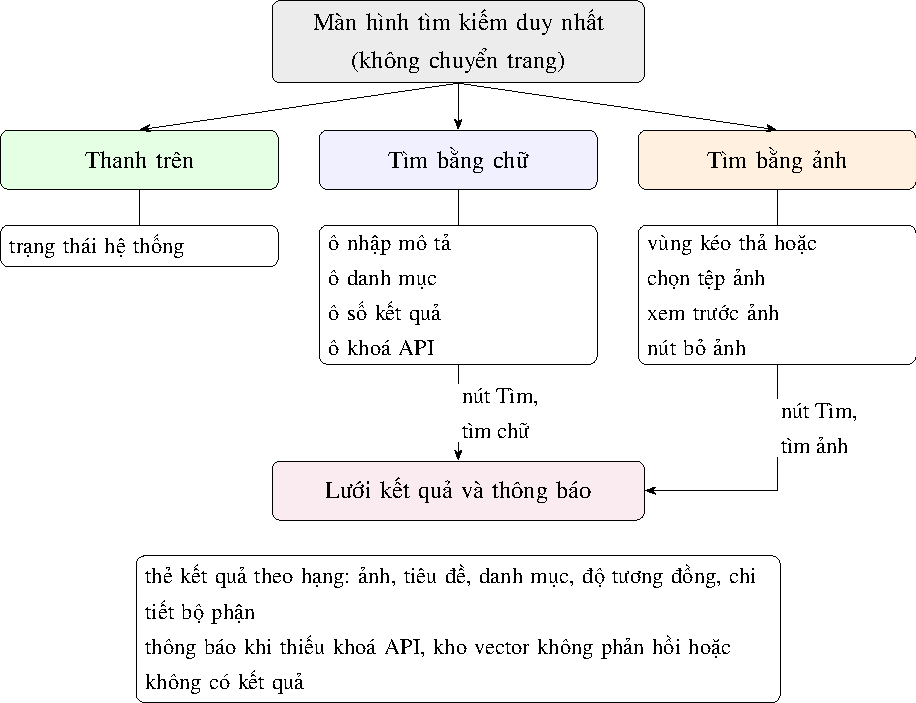
\includegraphics[width=0.66\textwidth]{graphics/fig_ch3_7.pdf}
\caption{Sơ đồ điều hướng của giao diện web}
\label{fig:c3_dieuhuong}
\end{figure}

Giao diện dùng một nút Tìm cho cả hai cách: khi đã chọn ảnh thì tìm theo ảnh, nếu không thì tìm theo chữ, nên người dùng không phải chuyển chế độ. Lỗi hiện bằng lời tiếng Việt theo từng nguyên nhân (Bảng~\ref{tab:c3_uc01} và \ref{tab:c3_uc02}).

\chapter{Cài đặt và xây dựng hệ thống}
\label{chap:cai_dat}

Chương này mô tả cách các thành phần thiết kế ở Chương~\ref{chap:thiet_ke} được cài đặt, và những giới hạn còn lại khi triển khai.

\section{Môi trường cài đặt}
\label{sec:moi-truong}

Bảng~\ref{tab:c4_moitruong} liệt kê môi trường của máy phát triển, có GPU Quadro T2000 4~GB, dùng để lập chỉ mục, đo độ trễ và chạy bản trình diễn. Ba bản trọng số tinh chỉnh được huấn luyện trên máy khác (Mục~\ref{sec:tinh-chinh}).

\begin{table}[H]
\centering
\caption{Môi trường cài đặt trên máy phát triển}
\label{tab:c4_moitruong}
\small
\renewcommand{\arraystretch}{1.15}
\begin{tabularx}{\textwidth}{@{}p{4.5cm} p{3.7cm} X@{}}
\toprule
\textbf{Thành phần} & \textbf{Phiên bản} & \textbf{Vai trò} \\
\midrule
GPU & Quadro T2000, 4~GB & Lập chỉ mục và mã hoá truy vấn \\
PyTorch & 2.5.1 (CUDA 12.1) & Suy luận trên máy phát triển \\
Transformers~\cite{wolf2020transformers} & 4.57.6 & Nạp SigLIP 2, SigLIP 1 và ViSigLIP-OT \\
PEFT~\cite{mangrulkar2022peft} & 0.20.0 & Tham số bổ sung (adapter) LoRA và DoRA \\
sentence-transformers~\cite{reimers2019sbert} & 5.1.0 & Nạp CLIP \\
rank-bm25~\cite{brown2020rankbm25} & 0.2.2 & Phương pháp đối chứng BM25 \\
Qdrant~\cite{qdrantdocs}, máy chủ và máy khách & 1.19.0 & Kho vector của bản trình diễn \\
\bottomrule
\end{tabularx}
\end{table}

\section{Nạp và chuẩn hoá dữ liệu}
\label{sec:nap-du-lieu}

Dữ liệu lấy từ Fashionpedia~\cite{jia2020fashionpedia}, bản sao trên Hugging Face, gồm 45.623 ảnh huấn luyện và 1.158 ảnh xác thực, tổng cộng 46.781 ảnh. Bản này chỉ có danh mục và hộp bao, không có màu hay chất liệu. Khi nạp, nhóm tính mã băm cảm nhận (pHash) của từng ảnh và loại 365 ảnh trùng hoặc không đọc được, còn 46.416 sản phẩm (số liệu hiện có không tách riêng hai lý do). Việc loại trùng diễn ra trước khi chia, nên hai ảnh giống hệt nhau không thể nằm ở hai tập khác nhau. Các sản phẩm còn lại được chia ngẫu nhiên theo tỷ lệ 70/15/15, với seed 42. Ảnh gần trùng, chẳng hạn cùng một sản phẩm chụp lại, có mã băm khác nên không bị loại. Nhóm chưa kiểm tra các ảnh gần trùng này, vì vậy tập kiểm tra có thể chứa ảnh gần giống ảnh huấn luyện.

Bảng~\ref{tab:c4_chia} cho thấy kết quả chia. Kho sản phẩm dùng để đánh giá và trình diễn là tập kiểm tra gồm 6.963 ảnh, chưa xuất hiện trong quá trình tinh chỉnh.

\begin{table}[H]
\centering
\caption{Ba tập dữ liệu sau khi lọc trùng và chia}
\label{tab:c4_chia}
\small
\renewcommand{\arraystretch}{1.15}
\begin{tabularx}{\textwidth}{@{}p{3.0cm} r@{\hspace{1.5em}}X@{}}
\toprule
\textbf{Tập} & \textbf{Số sản phẩm} & \textbf{Vai trò} \\
\midrule
Huấn luyện & 32.491 & Tinh chỉnh adapter \\
Xác thực & 6.962 & Chọn epoch tốt nhất \\
Kiểm tra & 6.963 & Kho sản phẩm được lập chỉ mục, đánh giá và trình diễn \\
\bottomrule
\end{tabularx}
\end{table}

Mỗi sản phẩm là một ảnh người mặc cả bộ trang phục. Tên sản phẩm liệt kê mọi món có trong ảnh (trung bình 2,95 món, nhiều nhất 11 món), còn trường danh mục chỉ ghi món đầu tiên. Trường danh mục dùng 46 loại của Fashionpedia, đã dịch tên sang tiếng Việt: 13 trang phục chính, 14 phụ kiện và 19 bộ phận hay chi tiết. Văn bản dùng để lập chỉ mục và cho BM25 chỉ gồm tên các danh mục, đã chuẩn hoá Unicode NFC và đưa về chữ thường, giữ nguyên dấu. Chú thích huấn luyện (caption) của mỗi ảnh gồm tên tiếng Việt của mọi danh mục trong ảnh, danh mục chính và tên các chi tiết bộ phận; không có màu, chất liệu hay giá.

\section{Bộ mã hoá ảnh và văn bản}
\label{sec:ma-hoa}

Mọi hệ tìm kiếm bằng vector dùng chung một giao diện mã hoá: nhận danh sách văn bản hoặc ảnh, trả về vector đã chuẩn hoá độ dài. Nhờ vậy muốn đổi mô hình chỉ cần sửa tệp cấu hình, phần còn lại của hệ thống giữ nguyên (Mục~\ref{sec:kien-truc}). Bảng~\ref{tab:c4_mahoa} tóm tắt các bộ mã hoá đã cài đặt (dòng cuối là bộ mã hoá mô phỏng, dùng khi kiểm thử và chạy cấu hình mặc định).

\begin{table}[H]
\centering
\caption{Các bộ mã hoá đã cài đặt}
\label{tab:c4_mahoa}
\small
\renewcommand{\arraystretch}{1.15}
\begin{tabularx}{\textwidth}{@{}p{3.6cm} r p{3.0cm} X@{}}
\toprule
\textbf{Bộ mã hoá} & \textbf{Số chiều} & \textbf{Giới hạn văn bản} & \textbf{Ghi chú} \\
\midrule
SigLIP 2~\cite{tschannen2025siglip2} & 768 & Đệm đến 64 token & Mô hình chính; mặc định chạy bf16 \\
CLIP ViT-B/32~\cite{radford2021clip} & 512 & 77 token & Đối chứng zero-shot \\
ViSigLIP-OT~\cite{viclipot2026} & 768 & Theo mô hình & Chạy trên CPU vì vector ảnh ra giá trị NaN trên GPU \\
SigLIP 1~\cite{zhai2023siglip} & 768 & Đệm đến 64 token & Ảnh đầu vào 256$\times$256 pixel, trong khi SigLIP 2 dùng 224$\times$224 \\
Bộ mã hoá mô phỏng & 64 & Không giới hạn & Chỉ dùng để kiểm thử và chạy cấu hình mặc định \\
\bottomrule
\end{tabularx}
\end{table}

SigLIP 2 và SigLIP 1 dùng chung một đoạn mã nạp, chỉ khác tên bản trọng số, nên so sánh hai mô hình này không tách được ảnh hưởng của kiến trúc khỏi độ phân giải ảnh. Khi nhận đường dẫn tới thư mục adapter, đoạn mã này gắn adapter LoRA hoặc DoRA lên mô hình gốc và nối tên adapter vào tên cấu hình tìm kiếm. Bộ mã hoá ảnh và bộ mã hoá văn bản luôn xuất vector đã chuẩn hoá $L_2$ ở độ chính xác 32 bit.

\section{Kho vector và chỉ mục}
\label{sec:kho-vector}

Bản trình diễn dùng Qdrant với khoảng cách cosine và chỉ mục HNSW~\cite{malkov2020hnsw}. Bộ sưu tập được tạo chỉ với số chiều và khoảng cách; các tham số HNSW giữ mặc định của máy chủ. Mỗi bản ghi trong Qdrant có mã định danh UUID5 sinh từ mã sản phẩm, nên lập chỉ mục lại sẽ ghi đè bản ghi cũ thay vì tạo bản trùng; kho trong bộ nhớ dùng thẳng mã sản phẩm làm định danh. Qdrant lưu toàn bộ thông tin sản phẩm cùng mỗi vector, nên API trả kết quả mà không cần tra thêm. Vector của hai bản trọng số khác nhau không so sánh được, nên mô hình gốc và mô hình tinh chỉnh dùng hai bộ sưu tập riêng.

Lập chỉ mục là bước chạy một lần, tách khỏi API: công cụ dòng lệnh mã hoá 6.963 ảnh kiểm tra rồi ghi vào Qdrant. Với SigLIP 2 chưa tinh chỉnh, bước này mất 1.336 s trên Quadro T2000 (khoảng 22 phút, 5,2 ảnh mỗi giây). Kho sản phẩm được mã hoá bằng ảnh thật, không bằng văn bản tên danh mục. Mọi phép đo ở Chương~\ref{chap:danh_gia} dùng kho vector trong bộ nhớ và tính cosine chính xác trên toàn bộ kho, không qua Qdrant; so sánh HNSW với tìm kiếm chính xác nằm ngoài phạm vi đánh giá (Mục~\ref{sec:han-che-danh-gia}).

\section{Tìm kiếm bằng văn bản và bằng ảnh}
\label{sec:tim-kiem}

Với các hệ vector, truy vấn chữ được mã hoá bằng bộ mã hoá văn bản rồi so với vector ảnh sản phẩm; kho trả về các sản phẩm gần nhất theo cosine. Truy vấn bằng ảnh đi qua bộ mã hoá ảnh và nằm trong cùng không gian vector với ảnh sản phẩm, nên không cần thêm thành phần nào. Đồ án đánh giá truy vấn bằng văn bản (Mục~\ref{sec:pham-vi}). Cả hai loại truy vấn đều có thể kèm bộ lọc danh mục khớp chính xác với trường danh mục của sản phẩm. Trên giao diện, sáu nút lọc nhanh (váy đầm, chân váy, sơ mi, áo khoác, quần dài, phụ kiện) mỗi nút điền sẵn đúng một tên danh mục; riêng nút phụ kiện chỉ ứng với danh mục mũ.

BM25~\cite{robertson2009bm25}, phương pháp đối chứng của đồ án, không dùng vector. Mỗi sản phẩm là một tài liệu gồm tên các danh mục tiếng Việt, tách theo khoảng trắng sau khi chuẩn hoá, với $k_1 = 1{,}5$ và $b = 0{,}75$. Kết quả của hệ này được trình bày ở Chương~\ref{chap:danh_gia}.

\section{Tinh chỉnh mô hình}
\label{sec:tinh-chinh}

Nhóm giữ nguyên trọng số của SigLIP 2 và chỉ huấn luyện adapter LoRA~\cite{hu2022lora}, kèm thành phần tách độ lớn của DoRA~\cite{liu2024dora}. Adapter gắn vào bốn phép chiếu của khối chú ý (q, k, v và phép chiếu đầu ra) ở cả bộ mã hoá ảnh lẫn bộ mã hoá văn bản. Với hạng 8, số tham số huấn luyện là 1.253.376, chiếm 0,33\% mô hình; LoRA thường có 1.179.648 tham số (0,31\%).

Hàm mất mát là mất mát sigmoid theo cặp của SigLIP~\cite{zhai2023siglip}. Để huấn luyện với 256 mẫu mỗi lô mà vừa bộ nhớ, nhóm dùng GradCache~\cite{gao2021gradcache}: mỗi lô được chia thành các nhóm 32 mẫu, còn mất mát vẫn tính trên cả 256 mẫu. Kích thước nhóm chọn theo GPU 12~GB dự kiến trong đề cương. Từ epoch thứ 5, nhóm xếp lại mẫu để mỗi sản phẩm cùng lô với bốn sản phẩm gần nhất cùng danh mục, tính từ vector của mô hình ở thời điểm đó. Bốn sản phẩm này là mẫu âm khó (hard negative) trong lô 256 mẫu; mô hình không lấy mẫu âm khó nào từ ngoài lô. Chú thích chỉ chứa tên danh mục, nên một phần mẫu âm khó có chú thích giống hệt ảnh gốc; chúng vẫn bị coi là cặp sai dù thực chất khớp. Nhóm chưa đo tỷ lệ này. Do dữ liệu không có màu (Mục~\ref{sec:nap-du-lieu}), tiêu chí ``khác màu'' của đề cương không áp dụng được và mẫu âm khó chỉ dựa vào danh mục.

Bản trọng số tốt nhất được chọn theo Recall@5 trên tập xác thực, dùng chính tên các danh mục của sản phẩm làm truy vấn giả. Recall@5 này chỉ đạt 0,26 đến 0,28 vì nhiều ảnh có tên danh mục giống nhau mà chỉ ảnh gốc được tính là đúng; nó chỉ dùng để chọn epoch trong cùng một lần chạy, không dùng để so sánh các cấu hình. Nhóm huấn luyện đầy đủ ba cấu hình: hệ DoRA (có mẫu âm khó, 3,08 giờ), LoRA thường và DoRA không có mẫu âm khó. Ba cấu hình chạy vào ba ngày khác nhau, trên máy của một thành viên khác với máy phát triển. Nhật ký không ghi cấu hình máy, phiên bản phần mềm hay kiểu số (bf16 hoặc fp32), nên thời gian huấn luyện chỉ mang tính tham khảo. Chi phí tài nguyên được bàn ở Chương~\ref{chap:danh_gia}.

\section{Công cụ đánh giá}
\label{sec:cong-cu-danh-gia}

Các chỉ số xếp hạng, hệ số Cohen's $\kappa$ và kiểm định bootstrap ghép cặp theo truy vấn~\cite{efron1993bootstrap} được tự cài đặt và kiểm bằng ví dụ tính tay; định nghĩa nằm ở Mục~\ref{sec:chi-so-danh-gia}. Nhãn được gán qua một máy chủ web cục bộ, mỗi người chấm nhận một phần việc riêng.

\section{Các tham số chính}
\label{sec:tham-so}

Bảng~\ref{tab:c4_thamso} gom các siêu tham số huấn luyện và kiểm định bootstrap; tham số của dữ liệu, tìm kiếm và API đã nêu ở các mục trên và ở Chương~\ref{chap:thiet_ke}.

\begin{table}[H]
\centering
\caption{Các tham số chính của hệ thống}
\label{tab:c4_thamso}
\footnotesize
\renewcommand{\arraystretch}{1.15}
\begin{tabularx}{\textwidth}{@{}p{4.6cm} p{4.4cm} X@{}}
\toprule
\textbf{Tham số} & \textbf{Giá trị} & \textbf{Cơ sở lựa chọn} \\
\midrule
Hạng LoRA, $\alpha$, dropout & 8, 16, 0,1 & Giữ giá trị trong đề cương \\
Vị trí gắn adapter & Bốn phép chiếu chú ý, hai bộ mã hoá & Giữ giá trị trong đề cương \\
Tốc độ học & $10^{-4}$, giảm theo cosine & Giữ giá trị trong đề cương \\
Khởi động, suy giảm trọng số & 500 bước, 0,01 & Khởi động chiếm khoảng 39\% trong 1.270 bước \\
Nhóm GradCache, lô huấn luyện & 32 và 256 & Xem Mục~\ref{sec:tinh-chinh} \\
Số epoch, dừng sớm & 10, dừng sau 2 epoch không cải thiện & Theo đề cương; bản trọng số chọn theo Recall@5 trên tập xác thực \\
Mẫu âm khó & 4 láng giềng cùng lô, từ epoch 5 & Giữ giá trị trong đề cương \\
Kiểm định bootstrap & 10.000 lần lặp, seed 42 & Độ phân giải $p$ tối thiểu $10^{-4}$ \\
\bottomrule
\end{tabularx}
\end{table}

\section{API và giao diện web}
\label{sec:api-giao-dien}

API web có các endpoint ở Bảng~\ref{tab:c4_api}. Khi khởi động, dịch vụ đọc tệp cấu hình để dựng bộ tìm kiếm một lần; tệp này quy định bộ mã hoá, kho vector và cách xếp hạng. Cấu hình mặc định dùng bộ mã hoá mô phỏng và 20 sản phẩm minh hoạ nên chạy được trên máy không có GPU; hai cấu hình còn lại dùng SigLIP 2 trên Qdrant, một cấu hình có thêm adapter tinh chỉnh. API không lập chỉ mục lại khi khởi động nếu cấu hình không khai báo danh sách sản phẩm.

\begin{table}[H]
\centering
\caption{Các endpoint của API web}
\label{tab:c4_api}
\small
\renewcommand{\arraystretch}{1.15}
\begin{tabularx}{\textwidth}{@{}p{4.4cm} p{2.4cm} X@{}}
\toprule
\textbf{Endpoint} & \textbf{Phương thức} & \textbf{Chức năng} \\
\midrule
\texttt{/search} & POST & Tìm bằng văn bản, kèm số kết quả và bộ lọc danh mục \\
\texttt{/search/image} & POST & Tìm bằng ảnh tải lên, kèm bộ lọc danh mục \\
\texttt{/health} & GET & Trạng thái, tên bộ tìm kiếm, số sản phẩm đã lập chỉ mục \\
\texttt{/image/\{đường dẫn\}} & GET & Ảnh sản phẩm trong kho \\
\texttt{/ui} & GET & Giao diện web chính \\
\texttt{/} & GET & Trang tìm kiếm dự phòng, nhúng sẵn trong mã \\
\bottomrule
\end{tabularx}
\end{table}

Giao diện web \texttt{/ui} là một trang tĩnh, một màn hình. Người dùng gõ mô tả bằng tiếng Việt hoặc kéo thả một ảnh, lọc theo danh mục và chọn số kết quả. Giao diện mặc định hiển thị 12 kết quả và cho chọn từ 1 đến 100. Khi gọi API trực tiếp mà không nêu số kết quả, API trả 10. Kết quả là lưới thẻ gồm ảnh, thứ hạng, tên, độ tương đồng và các nhãn chi tiết.

Trang \texttt{/} là bản dự phòng chỉ có ô nhập, khoá API và danh sách kết quả, gọi cùng endpoint \texttt{/search}. Các mã lỗi 413, 422 và 501 của tìm bằng ảnh nêu ở Chương~\ref{chap:thiet_ke}.

Giao diện đang chạy hệ DoRA trên 6.963 sản phẩm của tập kiểm tra hiện ở Hình~\ref{fig:c4_ui}. Với truy vấn ``áo len dệt kim xám'' lấy từ bộ đánh giá, ba kết quả đầu là áo len, kết quả thứ tư thì không. Hình chỉ minh hoạ giao diện, không phải bằng chứng về chất lượng tìm kiếm; chú thích huấn luyện không có màu (Mục~\ref{sec:nap-du-lieu}), nên truy vấn màu được bàn riêng ở Chương~\ref{chap:danh_gia}.

\begin{figure}[H]
\centering
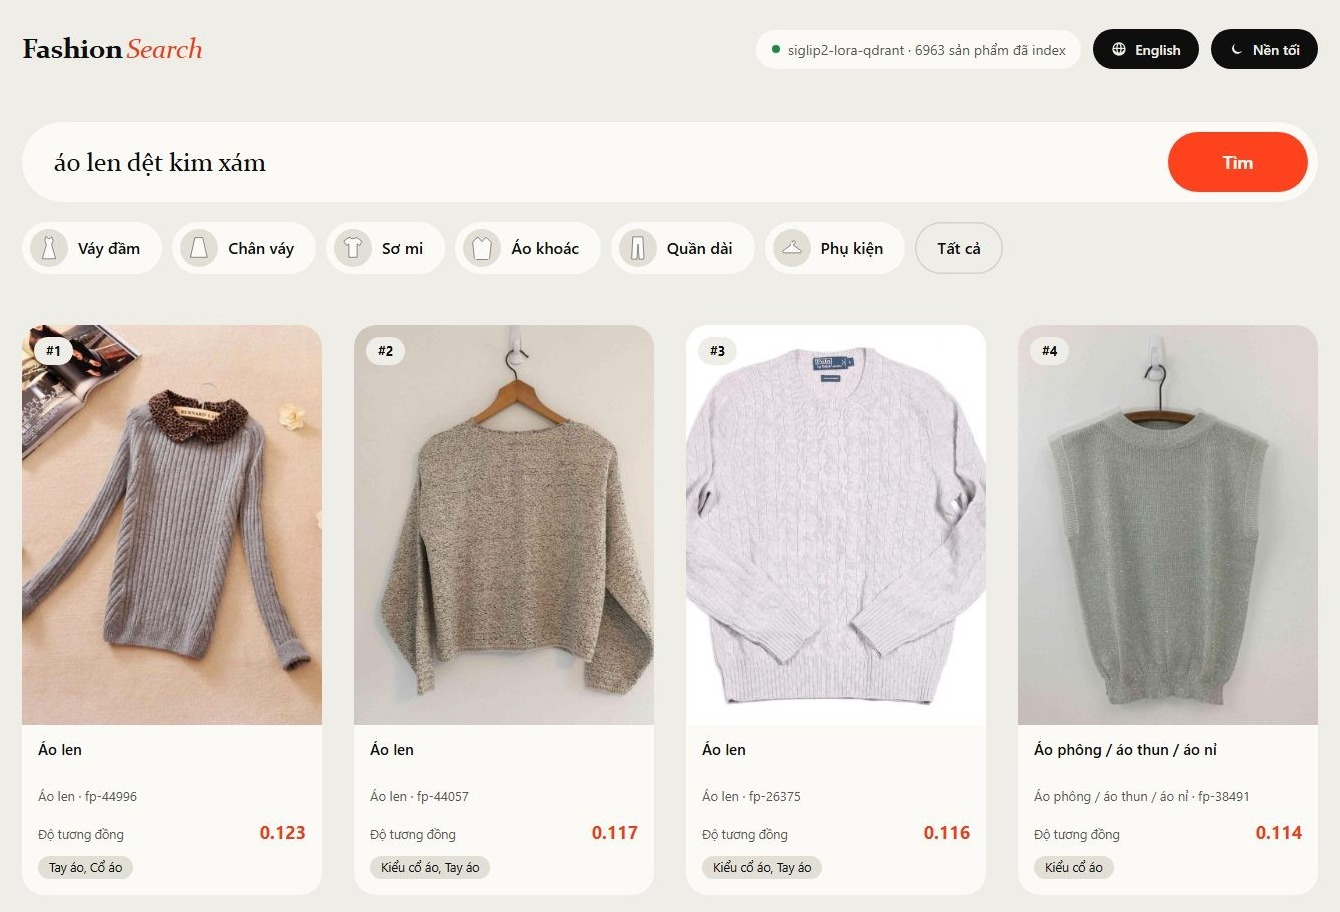
\includegraphics[width=\textwidth]{graphics/ui_ch4_sang_gon.jpg}
\caption{Màn hình tìm kiếm với truy vấn ``áo len dệt kim xám'', đã lược vùng tải ảnh}
\label{fig:c4_ui}
\end{figure}

Giao diện có hai ngôn ngữ (tiếng Việt, tiếng Anh) và hai chế độ màu (nền sáng, nền tối); trình duyệt ghi nhớ lựa chọn cho lần mở sau. Màn hình ban đầu, trước khi tìm, hiện ở cả bốn tổ hợp ngôn ngữ và chế độ màu trên Hình~\ref{fig:c4_home}; ảnh chỉ lấy ô nhập truy vấn, hàng nút chọn nhanh và các ô danh mục, số kết quả, khoá API.

\begin{figure}[H]
\centering
\begin{subfigure}[t]{\textwidth}
\centering
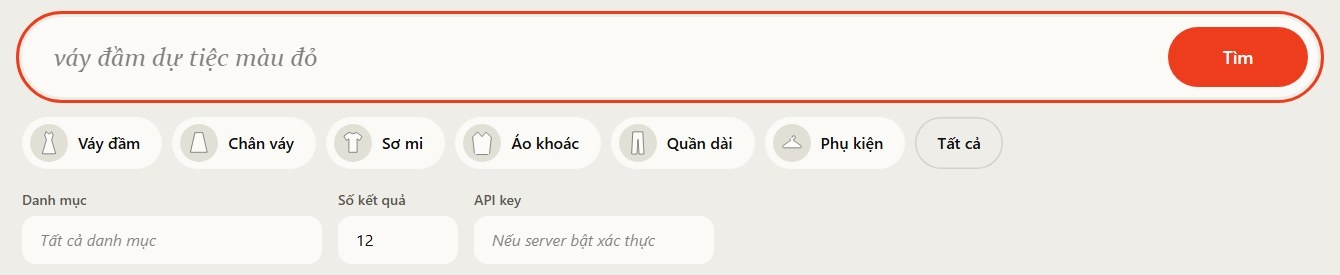
\includegraphics[width=\textwidth]{graphics/home_vi_light_cat.jpg}
\caption{Tiếng Việt, nền sáng}
\end{subfigure}

\vspace{0.4em}
\begin{subfigure}[t]{\textwidth}
\centering
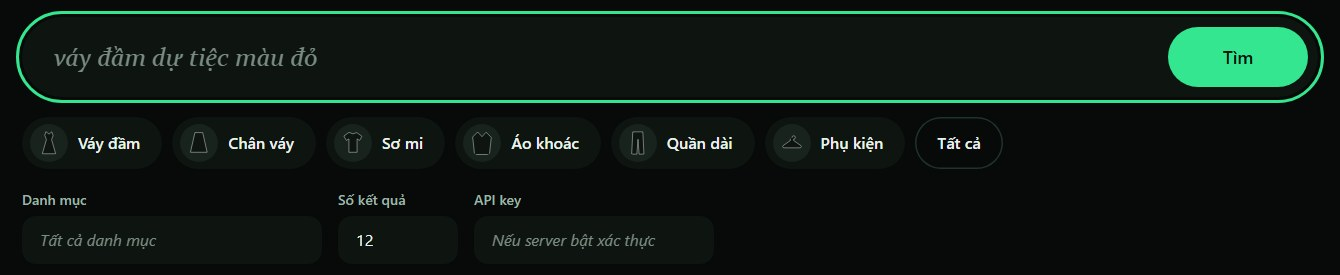
\includegraphics[width=\textwidth]{graphics/home_vi_dark_cat.jpg}
\caption{Tiếng Việt, nền tối}
\end{subfigure}

\vspace{0.4em}
\begin{subfigure}[t]{\textwidth}
\centering
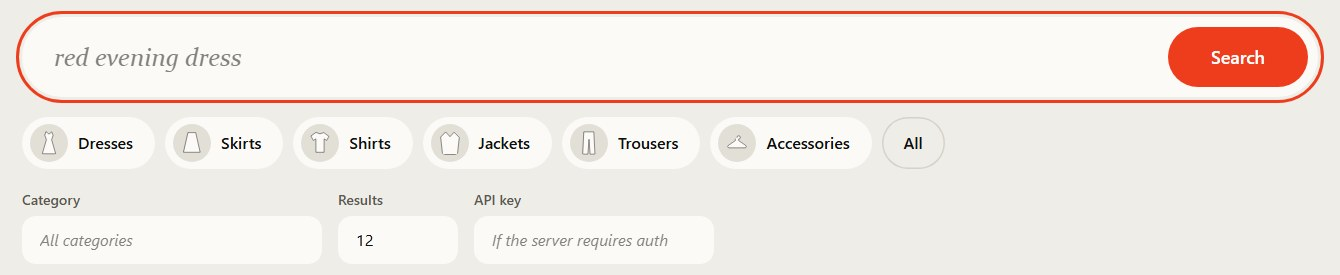
\includegraphics[width=\textwidth]{graphics/home_en_light_cat.jpg}
\caption{Tiếng Anh, nền sáng}
\end{subfigure}

\vspace{0.4em}
\begin{subfigure}[t]{\textwidth}
\centering
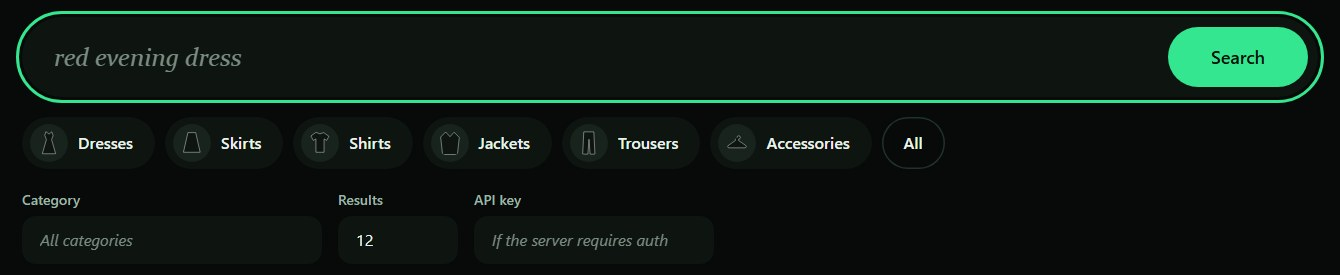
\includegraphics[width=\textwidth]{graphics/home_en_dark_cat.jpg}
\caption{Tiếng Anh, nền tối}
\end{subfigure}
\caption{Ô tìm, hàng nút chọn nhanh và các ô lọc ở màn hình ban đầu, hai ngôn ngữ và hai chế độ màu}
\label{fig:c4_home}
\end{figure}

Toàn bộ màn hình đầu tiên trong cửa sổ rộng được trình bày ở Hình~\ref{fig:c4_full}, với hai cấu hình đại diện (tiếng Việt nền sáng và tiếng Anh nền tối). Phần đầu trang có thanh trạng thái, cho biết bộ tìm kiếm đang chạy và số sản phẩm đã lập chỉ mục, cùng hai nút đổi ngôn ngữ và chế độ màu.

\begin{figure}[H]
\centering
\begin{subfigure}[t]{\textwidth}
\centering
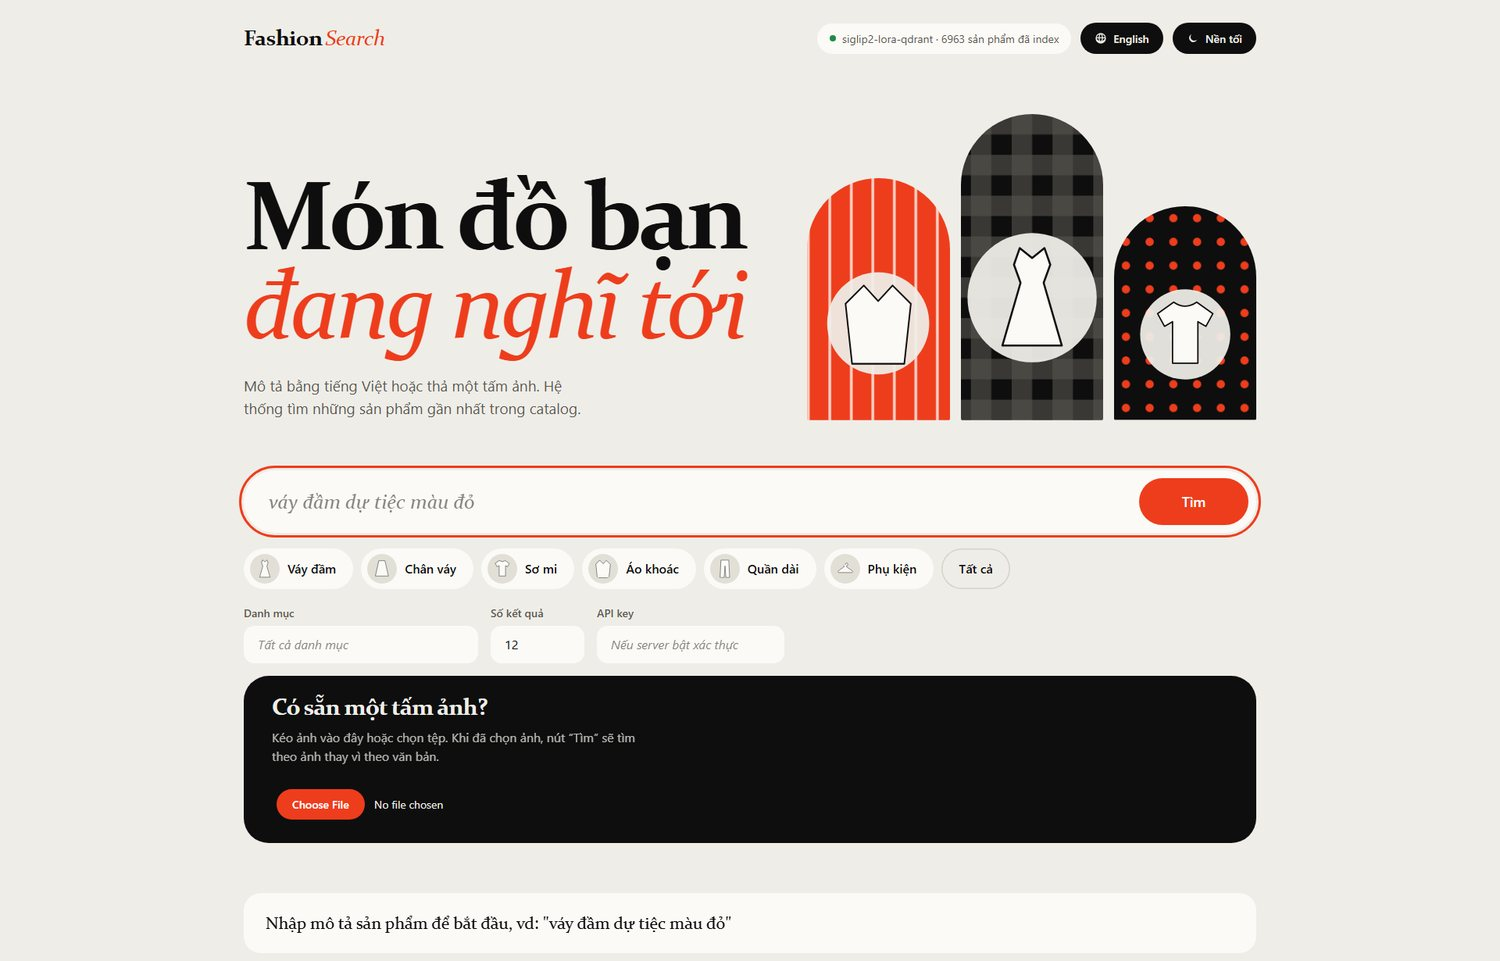
\includegraphics[width=\textwidth]{graphics/full_vi_light_cat.jpg}
\caption{Tiếng Việt, nền sáng}
\end{subfigure}

\vspace{0.6em}
\begin{subfigure}[t]{\textwidth}
\centering
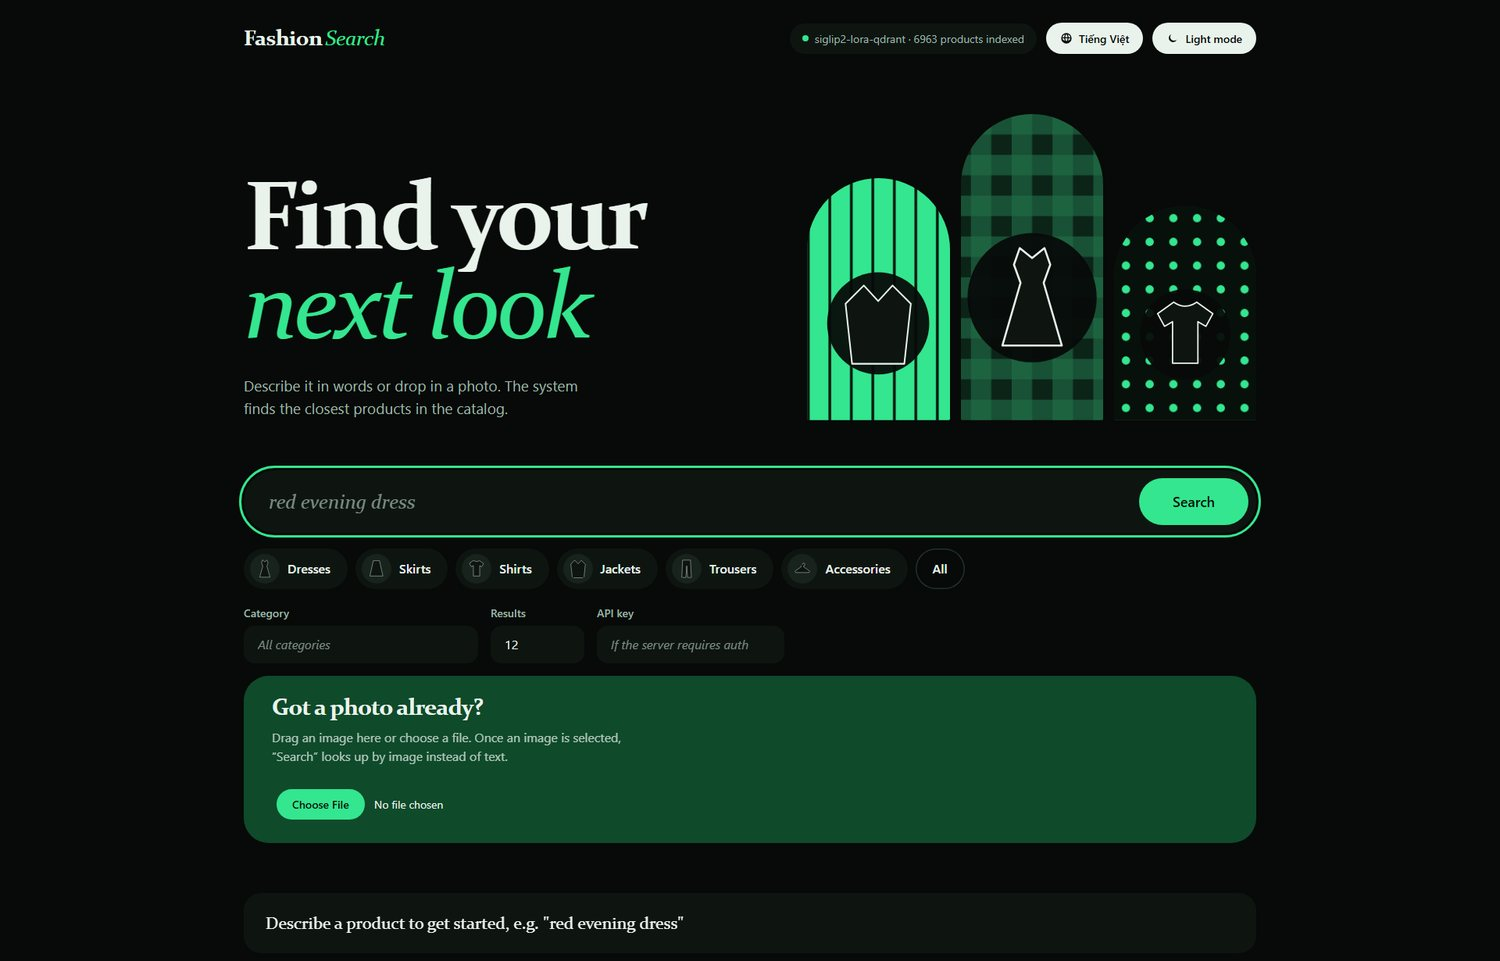
\includegraphics[width=\textwidth]{graphics/full_en_dark_cat.jpg}
\caption{Tiếng Anh, nền tối}
\end{subfigure}
\caption{Màn hình đầu tiên của giao diện web trong cửa sổ rộng, trước khi gửi truy vấn}
\label{fig:c4_full}
\end{figure}

\section{Triển khai và giới hạn}
\label{sec:trien-khai}

\subsection{Triển khai}

Hệ thống chạy trên một máy. Qdrant chạy bằng tệp thực thi gốc phiên bản 1.19.0; tệp mô tả container trong mã nguồn khai báo phiên bản 1.12.4, nên tổ hợp bản container này với máy khách 1.19.0 chưa được thử. Sau khi lập chỉ mục một lần, dịch vụ nạp mô hình rồi nhận truy vấn tại cổng cục bộ.

\subsection{Giới hạn hiện tại}

\begin{itemize}
\item Độ trễ: hệ DoRA chưa đạt chỉ tiêu 200 ms của đề cương trên máy đo (Mục~\ref{sec:danh-gia-dau-ra}).
\item Thực nghiệm: mỗi cấu hình chỉ huấn luyện một lần, với seed 42 (Chương~\ref{chap:danh_gia}).
\item Kiểm thử: bộ kiểm thử tự động gồm 21 tệp với 246 phép kiểm thử, đều đạt ở lần chạy mặc định. Thêm 13 phép kiểm thử cần GPU hoặc Qdrant không nằm trong lần chạy này và chưa được chạy lại trên phiên bản cuối.
\end{itemize}

\subsection{Bảo mật}

Khoá API là tuỳ chọn. Nếu không đặt biến môi trường tương ứng, hai endpoint tìm kiếm mở công khai; nếu đặt, yêu cầu phải mang khoá đúng trong tiêu đề, yêu cầu sai khoá bị từ chối với mã 401. Hệ thống so sánh khoá bằng phép so chuỗi thông thường, nên chưa phòng được tấn công dựa trên thời gian phản hồi.

Endpoint ảnh, trang \texttt{/ui} và trang \texttt{/} công khai theo thiết kế. Endpoint ảnh chặn đường dẫn có thành phần lên thư mục cha, đường dẫn tuyệt đối và tệp không phải ảnh. Cả hai trang hiển thị văn bản từ máy chủ dưới dạng chữ thuần, không chèn mã đánh dấu. Lỗi mất kết nối đến Qdrant trả về mã 503 với thông báo cố định, không lộ địa chỉ hay khoá.

Hệ thống chỉ có xác thực bằng một khoá API tuỳ chọn, chưa có giới hạn tốc độ, TLS, phân quyền theo người dùng hay nhật ký truy cập, nên chỉ chạy cục bộ. Qdrant chạy cục bộ không có khoá. Dữ liệu là bộ Fashionpedia công khai, không chứa dữ liệu cá nhân.

\chapter{Kiểm thử và đánh giá}
\label{chap:danh_gia}

Chương này trình bày kế hoạch kiểm thử (Mục~\ref{sec:ke-hoach-kiem-thu}), chất lượng tìm kiếm của các cấu hình (Mục~\ref{sec:danh-gia-cot-loi}) và độ trễ cùng chi phí (Mục~\ref{sec:danh-gia-dau-ra}). Tiếp theo là phân tích lỗi và đối soát nhãn (Mục~\ref{sec:phan-tich-loi}), phần trả lời các câu hỏi nghiên cứu (Mục~\ref{sec:tra-loi-ch}) và hạn chế của đánh giá (Mục~\ref{sec:han-che-danh-gia}).

\section{Kế hoạch kiểm thử}
\label{sec:ke-hoach-kiem-thu}

Kiểm thử diễn ra ở ba mức. Mức thứ nhất là kiểm thử tự động cho phần mềm, gồm 21 tệp với 222 hàm kiểm thử (đếm tĩnh; số ca thực tế nhiều hơn vì có tham số hoá). Lần chạy mặc định có 246 ca đạt, không ca nào lỗi. Có 13 ca cần GPU, cần Qdrant hoặc chạy lâu nên không nằm trong lần chạy này, và chưa rõ chúng có đạt trên phiên bản mã cuối hay không. Độ phủ mã chưa được đo.

Mức thứ hai là đánh giá chất lượng tìm kiếm trên 155 truy vấn tiếng Việt. Mức thứ ba là đo độ trễ của từng cấu hình. Bảng~\ref{tab:kt} liệt kê các hạng mục, yêu cầu phi chức năng tương ứng (Bảng~\ref{tab:c3_nfr}) và trạng thái.

\begin{table}[H]
\centering
\caption{Kế hoạch kiểm thử, yêu cầu phi chức năng tương ứng và trạng thái thực hiện}
\label{tab:kt}
\footnotesize
\renewcommand{\arraystretch}{1.05}
\begin{tabularx}{\textwidth}{@{}l >{\raggedright\arraybackslash}X l >{\raggedright\arraybackslash}p{4.6cm}@{}}
\toprule
\textbf{Mã} & \textbf{Đối tượng kiểm và cách kiểm} & \textbf{NFR} & \textbf{Kết quả} \\
\midrule
KT01 & Bộ chỉ số (Recall, MRR, nDCG, $\kappa$, bootstrap): 15 hàm kiểm thử đối chiếu giá trị tính tay & NFR04 & Đạt \\
KT02 & API web (truy vấn chữ và ảnh, ràng buộc đầu vào, khoá truy cập, lỗi kho vector): 28 hàm kiểm thử, không qua trình duyệt & NFR06, NFR07 & Đạt \\
KT03 & Lập chỉ mục, bảng đăng ký thành phần, công cụ gán nhãn, kiểm định, phân tích lỗi: 65 hàm kiểm thử & NFR03, NFR05 & Đạt \\
KT04 & Chất lượng của năm hệ chính: 155 truy vấn, nhãn của người chấm & NFR04 & Đã đo (Mục~\ref{sec:so-sanh-cau-hinh}) \\
KT05 & Ablation các trục 1, 2, 3 và 7 & -- & Đã đo bốn trục (Mục~\ref{sec:ablation}) \\
KT06 & Kiểm định thống kê: bootstrap ghép cặp, 10.000 lần lặp & -- & Đã làm (Mục~\ref{sec:kiem-dinh}) \\
KT07 & Độ trễ và chi phí: 155 truy vấn, từng truy vấn một & NFR01 & Đã đo; hệ DoRA chưa đạt chỉ tiêu 200~ms \\
KT08 & Đối soát nhãn tự động: đếm lại tệp nhãn, tính lại theo bộ lọc đã sửa & -- & Phát hiện lỗi ở bộ lọc (Mục~\ref{sec:doi-soat-nhan}) \\
\bottomrule
\end{tabularx}
\end{table}

Đối chiếu với yêu cầu phi chức năng của Chương~\ref{chap:thiet_ke}: NFR02 đến NFR07 đạt ở mức kiểm thử tự động; riêng NFR02 dựa trên lần chạy mặc định không có lỗi. NFR01 chưa đạt với hệ DoRA (Mục~\ref{sec:danh-gia-dau-ra}) và đạt với bốn hệ còn lại. NFR08 chưa đạt: catalog có 6.963 ảnh, thấp hơn ngưỡng 20.000 sản phẩm của đề cương.

\section{Đánh giá chất lượng tìm kiếm}
\label{sec:danh-gia-cot-loi}

\subsection{Dữ liệu và cách đo}
\label{sec:du-lieu-cach-do}

Catalog là tập kiểm tra gồm 6.963 ảnh Fashionpedia~\cite{jia2020fashionpedia}, chia sau khi lọc trùng và chưa từng dùng khi tinh chỉnh. Mỗi ảnh là một người mặc cả bộ: tiêu đề liệt kê trung bình 2,95 món (từ 1 đến 11 món), còn catalog chỉ lưu một danh mục chính cho mỗi ảnh. Văn bản đi kèm chỉ là tên các danh mục, không có màu, chất liệu hay mô tả của người bán.

Bộ truy vấn gồm 155 câu tiếng Việt do một người soạn, không lấy lại chú thích gốc của Fashionpedia, dài trung bình 6,62 từ, chia thành bốn nhóm. Nhóm A (46 câu) hỏi một thuộc tính, như ``áo len dệt kim xám''. Nhóm B (41 câu) hỏi nhiều thuộc tính, như ``áo len cổ tim mỏng màu than mặc mùa thu''. Nhóm C (33 câu) dùng từ địa phương hoặc từ mượn tiếng Anh, như ``giày sneaker trắng basic''. Nhóm D (35 câu) hỏi theo phong cách, như ``đồ dạo phố năng động mùa hè''.

Truy vấn được đưa vào mọi hệ nguyên văn, chỉ chuẩn hoá Unicode và chuyển về chữ thường; không dịch, không viết lại. Các hệ zero-shot (dùng nguyên mô hình đã huấn luyện sẵn) không có tham số nào chọn theo bộ này. Với hệ DoRA, nhóm chọn bản trọng số tốt nhất theo Recall@5 trên tập xác thực, dùng tên danh mục làm truy vấn giả; 155 truy vấn không tham gia việc chọn này.

Nhãn được lập theo quy trình ở Hình~\ref{fig:ch5-quytrinh}. Ở vòng 1, 10 kết quả đầu của bốn hệ đầu (BM25, CLIP, SigLIP 2 gốc, ViSigLIP-OT) được gộp thành một tập ứng viên, xáo trộn và ẩn tên hệ. Khi có hệ DoRA, vòng 2 bổ sung 10 kết quả đầu của hệ này, chỉ phần chưa có nhãn. Ba hệ ablation (LoRA thường, không mẫu âm khó, SigLIP 1) không nằm trong tập ứng viên nên một phần cặp của chúng chưa có nhãn (Mục~\ref{sec:ablation}). Mỗi cặp (truy vấn, ảnh) do hai người chấm độc lập theo thang 0 (không liên quan), 1 (liên quan một phần), 2 (liên quan chính xác). Một cặp được tính là liên quan khi điểm trung bình từ 1 trở lên; cặp hai người chấm $0$ và $2$ là liên quan, cặp $0$ và $1$ không liên quan.

Một phần cặp được tự động gán điểm 0 trước khi người chấm nhìn thấy. Vòng 1 gồm 6.079 cặp (4.011 do người chấm, 2.068 tự động); vòng 2 gồm 1.245 cặp (940 và 305). Tính chung hai vòng đầu: 7.324 cặp, trong đó 4.951 do người chấm và 2.373 tự động. Vòng 3 chỉ phục vụ ablation trục 2 và SigLIP 1: trong 1.262 cặp có 403 cặp tự động, 859 cặp còn lại không có người chấm.

Bộ lọc tự động gán điểm 0 cho cặp mà danh mục chính của ảnh không chứa từ khoá của truy vấn, để người chấm khỏi xem hàng nghìn cặp hiển nhiên sai. Với mỗi truy vấn, bộ lọc chọn danh mục đầu tiên có một từ dài hơn hai ký tự xuất hiện trong câu (khớp theo chuỗi con). Sau đó bộ lọc loại mọi ảnh mà danh mục chính không chứa từ đầu của tên danh mục đã chọn. Do mỗi ảnh chỉ lưu một danh mục chính và phép khớp theo chuỗi con quá lỏng, bộ lọc loại nhầm cả những ảnh có đúng món được hỏi. Các cặp tự động chiếm 32,4\% trong 7.324 cặp có nhãn của hai vòng đầu. Mục~\ref{sec:doi-soat-nhan} đối soát các cặp này; Mục~\ref{sec:sau-sua-loc} tính lại kết quả theo quy tắc đã sửa.

\begin{figure}[H]
\centering
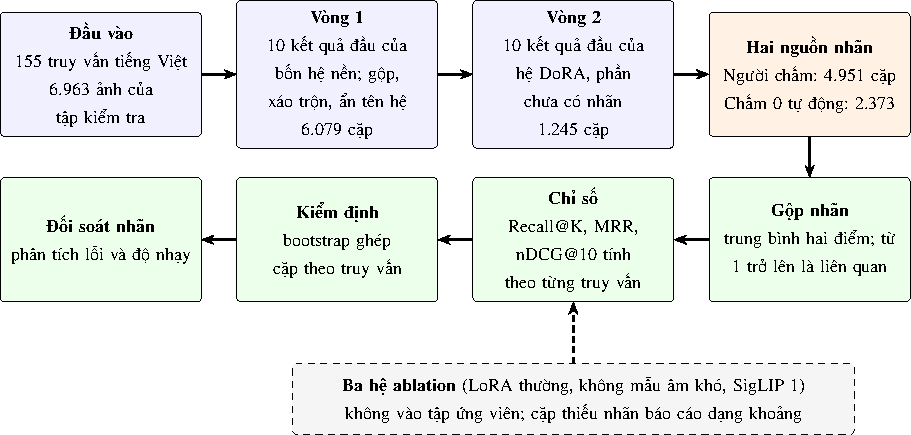
\includegraphics[width=\textwidth]{graphics/fig_ch5_1.pdf}
\caption{Quy trình đánh giá từ truy vấn đến kiểm định thống kê và đối soát nhãn}
\label{fig:ch5-quytrinh}
\end{figure}

Vòng 3 không phủ trục 1, nên trục 1 vẫn thiếu nhãn ở 102 cặp (6,6\%). Các số ở những mục sau dùng nhãn của hai vòng đầu; ô ablation dùng thêm nhãn vòng 3 và báo cáo dưới dạng khoảng (Mục~\ref{sec:ablation}).

Trong 4.951 cặp do người chấm, 4.655 cặp có hai người và 296 cặp có ba người; điểm của mỗi cặp là trung bình, người thứ ba không dùng để phân xử. Hệ số Cohen's $\kappa$ giữa từng đôi người chấm là 0,520 (3.545 cặp chung), 0,442 (1.219 cặp) và 0,441 (779 cặp). Cả ba ở mức trung bình theo thang $\kappa$ của Landis--Koch~\cite{landis1977kappa}, nên nhãn còn nhiễu, nhất là ở ranh giới giữa điểm 0 và 1.

Chỉ số gồm Recall@$K$, MRR và nDCG@10 (Mục~\ref{sec:chi-so-danh-gia}). Recall@$K$ là tỷ lệ trúng (hit rate), không phải recall của BEIR. nDCG@10 bỏ 16 truy vấn mà không ảnh nào trong tập ứng viên đạt điểm 1 trở lên. MRR xét 20 kết quả đầu nhưng chỉ 10 kết quả đầu được chấm đủ; nếu chỉ xét 10 kết quả, MRR lệch tối đa 0,0022 và thứ tự các hệ không đổi.

\subsection{So sánh các cấu hình}
\label{sec:so-sanh-cau-hinh}

Năm hệ có nhãn đầy đủ cho 10 kết quả đầu (Bảng~\ref{tab:ch1-he-thong}). BM25 chạy trên tên danh mục; CLIP, SigLIP 2 gốc và ViSigLIP-OT chạy zero-shot, riêng ViSigLIP-OT chạy trên CPU vì đầu ra bị NaN (giá trị không xác định) khi chạy trên GPU. Hệ DoRA là SigLIP 2 tinh chỉnh bằng DoRA với mẫu âm khó (Mục~\ref{sec:tinh-chinh}).

Bảng~\ref{tab:ket-qua-chinh} cho thấy cùng một thứ tự ở cả năm chỉ số: hệ DoRA, SigLIP 2 gốc, BM25, CLIP, ViSigLIP-OT. SigLIP 2 gốc có Recall@10 là 0,865, cao hơn BM25 (0,568) 29,7 điểm phần trăm, mà không cần dịch hay tinh chỉnh. Hai cột cuối là cận trên sau khi sửa bộ lọc chấm 0 tự động, với 641 cặp được tính lại (Mục~\ref{sec:sau-sua-loc}); các cột còn lại dùng nhãn hiện có. Giá trị in đậm là cao nhất mỗi cột.

\begin{table}[H]
\centering
\caption{Kết quả của năm hệ chính trên 155 truy vấn}
\label{tab:ket-qua-chinh}
\small
\renewcommand{\arraystretch}{1.12}
\setlength{\tabcolsep}{4pt}
\begin{tabular}{@{}l ccccc cc@{}}
\toprule
 & \multicolumn{5}{c}{\textbf{Nhãn hiện có}} & \multicolumn{2}{c}{\textbf{Cận trên}} \\
\cmidrule(lr){2-6}\cmidrule(lr){7-8}
\textbf{Hệ} & \textbf{R@1} & \textbf{R@5} & \textbf{R@10} & \textbf{MRR} & \textbf{nDCG@10} & \textbf{R@1} & \textbf{R@10} \\
\midrule
SigLIP 2 + DoRA & \textbf{0,697} & \textbf{0,852} & \textbf{0,884} & \textbf{0,766} & \textbf{0,684} & \textbf{0,839} & \textbf{1,000} \\
SigLIP 2 gốc & 0,490 & 0,774 & 0,865 & 0,606 & 0,449 & 0,613 & 0,987 \\
BM25 & 0,200 & 0,471 & 0,568 & 0,318 & 0,179 & 0,316 & 0,684 \\
CLIP ViT-B/32 & 0,168 & 0,381 & 0,426 & 0,252 & 0,139 & 0,206 & 0,555 \\
ViSigLIP-OT & 0,084 & 0,226 & 0,277 & 0,145 & 0,066 & 0,097 & 0,355 \\
\bottomrule
\end{tabular}
\end{table}

Tinh chỉnh tăng nhiều nhất ở các chỉ số nhạy với thứ hạng: Recall@1 tăng từ 0,490 lên 0,697 và nDCG@10 từ 0,449 lên 0,684, còn Recall@10 chỉ nhích từ 0,865 lên 0,884 (hiệu 0,019, $p = 0{,}240$; Mục~\ref{sec:kiem-dinh}). Mức tăng vì thế tập trung ở thứ hạng đầu; ở khả năng có ảnh đúng trong 10 kết quả chưa quan sát được khác biệt.

CLIP không hơn BM25 ở thứ hạng đầu, và ViSigLIP-OT thấp nhất ở mọi chỉ số. Nhóm chưa tìm ra nguyên nhân khiến ViSigLIP-OT thấp: có thể do lệch miền dữ liệu, cũng có thể do cách tích hợp mô hình chưa được đối chiếu với bản gốc. Kết luận vì vậy chỉ áp dụng cho thiết lập này.

Vị trí của BM25 và CLIP cần đọc kèm hướng lệch của nhãn. Bộ lọc và BM25 cùng dựa vào tên danh mục. Bộ lọc chỉ gán điểm 0, không bao giờ gán điểm cao, nên nó chỉ làm giảm điểm của các hệ có nhiều kết quả bị lọc. Trong 10 kết quả đầu, cặp mang nhãn tự động chiếm 20,3\% ở BM25 và 23,9\% ở hệ DoRA, còn ở SigLIP 2 gốc, CLIP và ViSigLIP-OT là 33,6\%, 39,3\% và 42,3\%. Các hệ nhìn ảnh, nhất là CLIP, vì vậy bị bất lợi hơn BM25, và việc BM25 cao hơn CLIP ở Recall@10 ($p = 0{,}003$) có thể một phần do nhãn.

Sau khi tính lại, BM25 vẫn cao hơn CLIP (Recall@10 là 0,684 so với 0,555), nhưng đó là cận trên và chưa qua người chấm. Ngược lại, SigLIP 2 gốc vượt BM25 dù nhãn không thiên về nó. Muốn đối chứng cần một tập truy vấn thứ hai có nhãn không bị bộ lọc can thiệp (Mục~\ref{sec:han-che-danh-gia}).

Theo nhóm truy vấn (Hình~\ref{fig:ch5-nhom}), nhóm D dễ nhất với mọi hệ: Recall@10 của hai hệ SigLIP 2 là 1,000 và của BM25 là 0,971. Số này đo độ rộng của truy vấn nhiều hơn khả năng hiểu phong cách, vì một câu như ``đồ đi biển thoải mái mùa hè'' có rất nhiều ảnh phù hợp. BM25 yếu nhất ở nhóm C (Recall@10 là 0,212). Hệ DoRA đạt 0,909 ở nhóm C và 0,804 ở nhóm A, nhưng khoảng tin cậy bootstrap 95\% của hai nhóm chồng nhau, nên chưa kết luận từ mượn dễ hơn từ thuần Việt.

\begin{figure}[H]
\centering
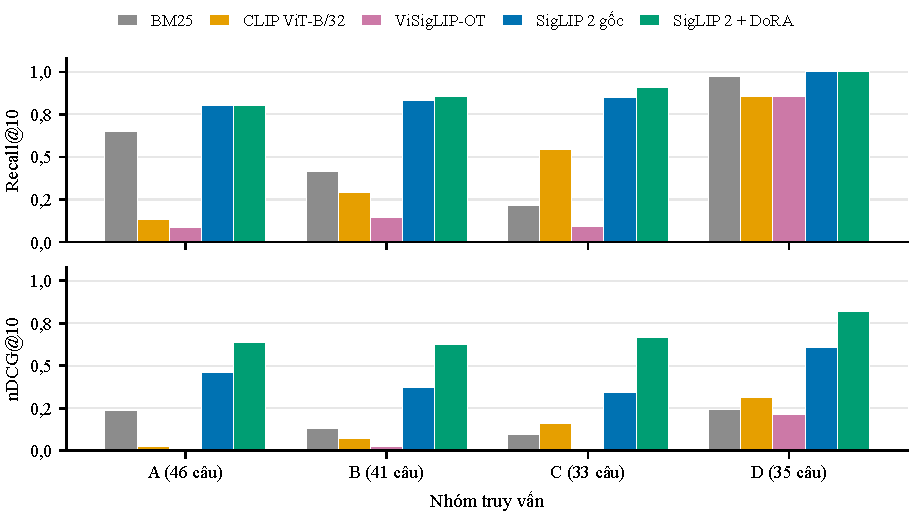
\includegraphics[width=\textwidth]{graphics/fig_ch5_3.pdf}
\caption{Recall@10 và nDCG@10 theo nhóm truy vấn}
\label{fig:ch5-nhom}
\end{figure}

\subsection{Các trục ablation}
\label{sec:ablation}

Đề cương nêu bảy trục ablation. Bốn trục đã chạy: trục 1 (DoRA so với LoRA thường), trục 2 (bật hoặc tắt mẫu âm khó), trục 3 (SigLIP 2 so với ViSigLIP-OT, xét bằng so sánh zero-shot ở Bảng~\ref{tab:ket-qua-chinh}) và trục 7 (SigLIP 1 so với SigLIP 2, chỉ suy luận). Ba trục 4, 5, 6 (hạng LoRA, kích thước lô hiệu dụng, vị trí gắn adapter) là hướng phát triển, dành cho giai đoạn sau. Mỗi cấu hình chỉ huấn luyện một lần.

Mỗi ô của Bảng~\ref{tab:ablation} chỉ đổi một yếu tố so với cấu hình tham chiếu. Vì ba hệ ablation không nằm trong tập ứng viên, một phần cặp trong 10 kết quả đầu của chúng chưa có nhãn. Các ô vì thế được báo cáo dưới dạng khoảng, dấu ``--'' nối hai cận: cận dưới coi mọi cặp chưa chấm là không liên quan, cận trên coi tất cả là liên quan. nDCG@10 không có cận trên hợp lệ nên không báo cáo cho các ô này.

\begin{table}[H]
\centering
\caption{Kết quả ablation trên 155 truy vấn}
\label{tab:ablation}
\footnotesize
\renewcommand{\arraystretch}{1.12}
\setlength{\tabcolsep}{4pt}
\begin{tabularx}{\textwidth}{@{}>{\raggedright\arraybackslash}X c c c c c@{}}
\toprule
\textbf{Cấu hình} & \textbf{R@1} & \textbf{R@5} & \textbf{R@10} & \textbf{MRR} & \textbf{Thiếu nhãn} \\
\midrule
SigLIP 2 gốc & 0,490 & 0,774 & 0,865 & 0,606 & 0\% \\
DoRA, mẫu âm khó (tham chiếu) & 0,697 & 0,852 & 0,884 & 0,766 & 0\% \\
Trục 1: LoRA thường & 0,690 & 0,832--0,839 & 0,884--0,923 & 0,760--0,771 & 6,6\% \\
Trục 2: không mẫu âm khó & 0,697 & 0,845--0,858 & 0,858--0,884 & 0,763--0,776 & 11,3\% \\
Trục 7: SigLIP 1 zero-shot & 0,316--0,645 & 0,548--0,826 & 0,710--0,890 & 0,427--0,738 & 44,5\% \\
\bottomrule
\end{tabularx}
\end{table}

Với trục 1, LoRA thường và DoRA chưa quan sát được khác biệt ở Recall@1 ($p = 0{,}82$) và MRR ($p = 0{,}41$). Recall@10 của LoRA thường chỉ là cận dưới 0,884 và có thể tới 0,923 vì 6,6\% cặp thiếu nhãn; giá trị $p = 1{,}00$ ở Recall@10 chỉ đúng cho cận dưới. Hai hệ trùng 92\% top-10 và hiệu Recall@1 chỉ 0,0065 (một truy vấn), nên với 155 truy vấn và một lần huấn luyện cho mỗi cấu hình thì chưa có bằng chứng DoRA hơn LoRA thường.

LoRA thường huấn luyện ít tham số hơn một chút (0,31\% so với 0,33\% mô hình) và mất 7.437,6 s so với 11.084,7 s, ngắn hơn 32,9\%. Với trục 2, Recall@1 giống hệt tham chiếu ($p = 1{,}00$; ở $K = 1$ không cặp nào thiếu nhãn) và MRR chưa quan sát được khác biệt ($p = 0{,}74$). Recall@10 thấp hơn (cận dưới 0,858 so với 0,884, $p = 0{,}037$), nhưng ô này thiếu 11,3\% nhãn và cận trên của nó bằng giá trị tham chiếu, nên chưa kết luận được. Bước đào mẫu âm khó làm huấn luyện lâu hơn 28,3\% (11.084,7 s so với 8.642,1 s).

Với trục 7, khoảng Recall@1 của SigLIP 1 ($[0{,}316;\,0{,}645]$) chứa giá trị của SigLIP 2 gốc (0,490) nhưng không chứa giá trị của hệ DoRA (0,697). Vì vậy SigLIP 1 thấp hơn hệ DoRA ở Recall@1; so với SigLIP 2 gốc thì chưa kết luận được. Ngoài ra ảnh đầu vào của SigLIP 1 là 256 pixel thay vì 224. Với trục 3, SigLIP 2 vượt ViSigLIP-OT (Recall@1 là 0,490 so với 0,084); chưa tách được phần do mô hình và phần do cách tích hợp.

\subsection{Kiểm định thống kê}
\label{sec:kiem-dinh}

Kiểm định dùng bootstrap ghép cặp theo truy vấn~\cite{efron1993bootstrap}: chọn lại 155 truy vấn có hoàn lại, 10.000 lần, seed 42, hai phía, mức $0{,}05$. Cách này thay cho McNemar vì MRR không phải chỉ số nhị phân và cả năm hệ chạy trên cùng 155 truy vấn. Giá trị $p$ ghi bằng $0$ trong tệp kết quả được viết là $p < 10^{-4}$, đúng độ phân giải của 10.000 lần lặp. SigLIP 1 bị loại khỏi kiểm định vì lúc chạy (trước vòng 3), 67\% cặp trong 10 kết quả đầu của nó chưa có nhãn. Giá trị $p$ so với nó khi đó phản ánh việc thiếu nhãn hơn là chất lượng của hệ. Kết quả nằm ở Bảng~\ref{tab:kiem-dinh}.

\begin{table}[H]
\centering
\caption{Kiểm định bootstrap ghép cặp trên 155 truy vấn}
\label{tab:kiem-dinh}
\small
\setlength{\tabcolsep}{4pt}
\renewcommand{\arraystretch}{1.12}
\begin{tabular}{@{}l r r r r r r@{}}
\toprule
 & \multicolumn{2}{c}{\textbf{Recall@1}} & \multicolumn{2}{c}{\textbf{Recall@10}} & \multicolumn{2}{c}{\textbf{MRR}} \\
\cmidrule(lr){2-3}\cmidrule(lr){4-5}\cmidrule(lr){6-7}
\textbf{So sánh} & $\Delta$ & $p$ & $\Delta$ & $p$ & $\Delta$ & $p$ \\
\midrule
DoRA $-$ SigLIP 2 gốc & $+0{,}206$ & $<10^{-4}$ & $+0{,}019$ & $0{,}240$ & $+0{,}160$ & $<10^{-4}$ \\
SigLIP 2 gốc $-$ BM25 & $+0{,}290$ & $<10^{-4}$ & $+0{,}297$ & $<10^{-4}$ & $+0{,}289$ & $<10^{-4}$ \\
SigLIP 2 gốc $-$ CLIP & $+0{,}323$ & $<10^{-4}$ & $+0{,}439$ & $<10^{-4}$ & $+0{,}355$ & $<10^{-4}$ \\
BM25 $-$ CLIP & $+0{,}032$ & $0{,}481$ & $+0{,}142$ & $0{,}003$ & $+0{,}066$ & $0{,}070$ \\
BM25 $-$ ViSigLIP-OT & $+0{,}116$ & $0{,}001$ & $+0{,}290$ & $<10^{-4}$ & $+0{,}173$ & $<10^{-4}$ \\
CLIP $-$ ViSigLIP-OT & $+0{,}084$ & $0{,}015$ & $+0{,}148$ & $0{,}002$ & $+0{,}107$ & $0{,}001$ \\
\bottomrule
\end{tabular}
\end{table}

Trong Bảng~\ref{tab:kiem-dinh}, $\Delta$ là hiệu của hệ thứ nhất trừ hệ thứ hai. Hệ DoRA tốt hơn SigLIP 2 gốc ở Recall@1 và MRR nhưng chưa quan sát được khác biệt ở Recall@10. SigLIP 2 gốc tốt hơn BM25 và CLIP ở cả ba chỉ số. ViSigLIP-OT thấp hơn cả BM25 và CLIP. BM25 và CLIP chưa phân biệt được ở Recall@1 và MRR. Bảng gồm 18 giá trị $p$ chưa hiệu chỉnh; theo ngưỡng Bonferroni $0{,}05/18 \approx 0{,}0028$, hai giá trị $0{,}003$ (BM25 so với CLIP ở Recall@10) và $0{,}015$ (CLIP so với ViSigLIP-OT ở Recall@1) chỉ là gợi ý.

\section{Độ trễ và chi phí}
\label{sec:danh-gia-dau-ra}

Độ trễ đo trên máy phát triển (GPU Quadro T2000 4~GB), với kho vector trong bộ nhớ, trên catalog 6.963 ảnh, từng truy vấn chữ một, lấy 20 kết quả đầu, bỏ 5 truy vấn khởi động. Mỗi truy vấn được đo ba thành phần: mã hoá truy vấn, tìm trong chỉ mục và tổng đầu-cuối. Chỉ tiêu của đề cương là dưới 200~ms cho một truy vấn trên một GPU. Đề cương tính cho GPU mạnh hơn máy đo, nên kết quả chỉ phản ánh máy này. Kết quả nằm ở Bảng~\ref{tab:do-tre}.

\begin{table}[H]
\centering
\caption{Độ trễ theo thành phần, p50 / p95 (ms)}
\label{tab:do-tre}
\small
\renewcommand{\arraystretch}{1.12}
\begin{tabular}{@{}l c c c c@{}}
\toprule
\textbf{Hệ} & \textbf{Thiết bị} & \textbf{Mã hoá truy vấn} & \textbf{Tìm trong chỉ mục} & \textbf{Đầu-cuối} \\
\midrule
BM25 & CPU & 0,01 / 0,03 & 8,68 / 15,69 & 14,67 / 24,13 \\
CLIP ViT-B/32 & GPU & 40,83 / 69,30 & 26,37 / 43,63 & 66,78 / 111,96 \\
SigLIP 2 gốc & GPU & 48,94 / 73,19 & 41,24 / 54,96 & 91,55 / 127,37 \\
ViSigLIP-OT & CPU & 71,38 / 87,80 & 48,12 / 56,88 & 118,25 / 146,45 \\
SigLIP 2 + DoRA & GPU & 193,59 / 663,59 & 48,61 / 127,51 & 245,57 / 746,32 \\
\bottomrule
\end{tabular}
\end{table}

Bảng~\ref{tab:do-tre} cho thấy bốn hệ đầu bảng đạt chỉ tiêu cả ở p50 lẫn p95. ViSigLIP-OT chậm nhất nhóm này (p95 là 146,45~ms) nhưng chạy trên CPU nên không so trực tiếp với các hàng GPU. Hệ DoRA không đạt: p50 là 245,57~ms và p95 là 746,32~ms. Thành phần chi phối là mã hoá truy vấn, với p50 là 193,59~ms (khoảng 4 lần SigLIP 2 gốc) và p95 là 663,59~ms (khoảng 9 lần). Adapter được nạp riêng chứ chưa gộp vào trọng số; nhóm chưa thử gộp nên chưa biết cách này có giảm được độ trễ hay không.

Lần huấn luyện tham chiếu của hệ DoRA (10 epoch trên 32.491 ảnh, lô hiệu dụng 256) mất 11.084,7 s, tức 3,08 giờ.

\section{Phân tích lỗi}
\label{sec:phan-tich-loi}

\subsection{Đối soát bộ lọc chấm 0}
\label{sec:doi-soat-nhan}

Cách bộ lọc hoạt động đã nêu ở Mục~\ref{sec:du-lieu-cach-do}. Đối soát đánh dấu 35 truy vấn bị bộ lọc ảnh hưởng, chia thành ba nhóm rời nhau.

\textbf{Phụ kiện (14 truy vấn, 406 cặp).} Ảnh người đeo kính, xách túi hay đi giày có danh mục chính là một món áo hoặc váy. Vì vậy chúng nhận điểm 0 ở các truy vấn kính, băng đô, cà vạt, đồng hồ, dây nịt, giày, túi và khăn choàng, dù tiêu đề ảnh có món được hỏi.

\textbf{Từ khoá giả (12 truy vấn, 393 cặp).} Bộ lọc khớp một từ ngắn nằm trong cụm khác và lấy nhầm danh mục. Từ ``dài'' trong ``tay dài'' kéo theo ``Quần dài''; từ ``tay'' trong ``găng tay'' kéo theo ``Áo choàng không tay''; từ ``váy'' trong ``váy hai dây'' kéo theo ``Chân váy''.

\textbf{Từ khoá đầm (9 truy vấn, 131 cặp).} Truy vấn viết ``đầm'' còn tên danh mục là ``Váy đầm'', nên từ đầu ``váy'' không có trong câu và truy vấn bị đánh dấu. Ở nhóm này bộ lọc chọn đúng loại sản phẩm. Nhóm này vẫn được giữ trong 35 truy vấn vì quy tắc đánh dấu chạy tự động, không để người viết quyết định truy vấn nào ở lại.

Như vậy bộ lọc gán nhãn sai ở 26 truy vấn (14 phụ kiện và 12 từ khoá giả; 799 cặp). Cả 18 truy vấn mà hệ DoRA trượt Recall@10 đều nằm trong 26 truy vấn này: 14 phụ kiện và 4 từ khoá giả (41, 57, 64, 148), không truy vấn nào thuộc nhóm đầm. SigLIP 2 gốc trượt 21 truy vấn, trong đó 19 nằm trong 35 truy vấn bị đánh dấu.

Người chấm có xem ảnh cả bộ ở 10 truy vấn phụ kiện (mã 15, 18, 22, 25, 26, 35, 40, 73, 75, 101; mũ, vớ, dù, ví, găng tay, khăn). Ở 6 trong số đó (18, 25, 35, 40, 73, 75) người chấm chỉ thấy các cặp đã lọt qua bộ lọc; 4 truy vấn còn lại (15, 22, 26, 101) không bị bộ lọc ảnh hưởng. Trong các cặp do người chấm xem, 82 trên 138 cặp (59,4\%) có món được hỏi trong tiêu đề được chấm liên quan, so với 6 trên 169 cặp (3,6\%) khi ảnh không có món đó. Mẫu này nghiêng về các món dễ thấy, nên tỷ lệ chỉ cho biết người chấm có thể chấp nhận ảnh cả bộ.

\subsection{Các truy vấn lỗi nặng nhất}
\label{sec:hai-muoi-loi}

Phân tích lấy hệ DoRA làm đối tượng, SigLIP 2 gốc làm mốc, $K = 10$, trên 20 truy vấn. Đó là 18 truy vấn mà hệ DoRA không có ảnh liên quan trong 10 kết quả đầu, cộng hai truy vấn mà hệ DoRA kém SigLIP 2 gốc nhiều nhất. Xem lại nguồn gốc các nhãn 0 cho thấy phần lớn do bộ lọc chứ không do người chấm: 16 trong 20 truy vấn có cả 10 kết quả đầu mang nhãn 0 tự động. Vì vậy nhóm không dùng các nguyên nhân gán bằng tay, như ``ảnh chứa nhiều sản phẩm'', làm kết luận. Ở ``áo sơ mi lụa tay dài công sở màu trắng ngà'' (41), bộ lọc khớp từ ``dài'' với danh mục ``Quần dài'' nên gán điểm 0 cho mọi ảnh không có quần dài. Ở ``giày cao gót đen'' (23), ảnh đứng đầu có danh mục chính là đầm nên nhận điểm 0 dù người mẫu đi giày.

\subsection{Kết quả sau khi sửa bộ lọc}
\label{sec:sau-sua-loc}

Vì chưa thể chấm lại toàn bộ các cặp bị lọc, nhóm tính lại theo một quy tắc đã sửa. Với 35 truy vấn bị đánh dấu, nhóm gán thủ công danh mục được hỏi sau khi đã xem các ca lỗi. Một cặp bị chấm 0 tự động được tính là liên quan nếu danh mục đó có trong tiêu đề ảnh, kể cả khi không phải danh mục chính. Có 641 cặp được tính lại (398 ở truy vấn phụ kiện, 238 ở từ khoá giả, 5 ở từ khoá đầm); các cặp còn lại giữ nhãn cũ.

Hai cột cuối của Bảng~\ref{tab:ket-qua-chinh} là kết quả tính lại. Đó là cận trên chứ không phải số đo: quy tắc coi mọi ảnh chứa món được hỏi là liên quan, trong khi người chấm chỉ chấp nhận 59,4\% số đó ở các truy vấn phụ kiện đã chấm. Thứ tự năm hệ không đổi ở cả hai chỉ số. Bootstrap với nhãn đã sửa cho cùng kết luận về hai hệ đầu bảng: hệ DoRA tốt hơn ở Recall@1 ($+0{,}226$, $p < 10^{-4}$) và chưa quan sát được khác biệt ở Recall@10 ($+0{,}013$, $p = 0{,}272$).

Mức lỗi do nhãn chưa định lượng được. Mỗi truy vấn trong 18 truy vấn trượt có từ 3 đến 10 ảnh chứa món được hỏi nhưng bị chấm 0 tự động ở 10 kết quả đầu. Nếu người chấm chấp nhận mọi ảnh đó, cả 18 truy vấn đều có ảnh liên quan. Nếu chỉ chấp nhận 59,4\% như ở các truy vấn phụ kiện đã chấm, số truy vấn có ảnh đúng nằm trong khoảng 11 đến 18, tuỳ mức độ các ảnh của cùng một truy vấn được chấp nhận cùng nhau. Riêng tỷ lệ 59,4\% dao động từ 0,33 đến 1,00 giữa các truy vấn.

Bảng chính là kết quả trên cả 155 truy vấn. Nhóm bỏ 35 truy vấn do bộ lọc đánh dấu để làm phân tích độ nhạy. Tập này được chọn sau khi đã xem các ca lỗi, nên không thay thế bảng chính và không phải kết quả của hệ thống. Trên 120 truy vấn còn lại, hệ DoRA đạt Recall@1 là 0,825 và Recall@10 là 1,000; SigLIP 2 gốc đạt 0,542 và 0,983. Nếu chỉ bỏ 26 truy vấn bị lọc sai (còn 129 truy vấn), Recall@1 là 0,822 với hệ DoRA và 0,558 với SigLIP 2 gốc. Giữ hay bỏ 9 truy vấn đầm vì vậy không đổi kết luận.

Tập 120 cũng chưa phải tập sạch: 60 truy vấn trong đó còn 1.187 cặp chấm 0 tự động, và 322 cặp ở 57 truy vấn có nguyên tên danh mục nằm trong tiêu đề ảnh dù danh mục chính khác. Đó là cận trên số cặp có thể bị gán điểm 0 oan, chưa phải số lỗi đã xác nhận.

Có hai điều không đổi. Thứ nhất, catalog thiếu ảnh phụ kiện đứng riêng: không ảnh nào trong tập kiểm tra lấy giày, túi, kính mắt, đồng hồ hay dây nịt làm danh mục chính. Thứ hai, lỗi của mô hình ở thứ hạng đầu chưa tách được khỏi lỗi nhãn: ngay với cận trên vẫn còn 25 truy vấn (16,1\%) chưa có ảnh đúng ở vị trí đầu.

\section{Trả lời các câu hỏi nghiên cứu}
\label{sec:tra-loi-ch}

\textbf{CH1. Tìm kiếm bằng biểu diễn chung đa mô thức dùng zero-shot (SigLIP~2, CLIP, ViSigLIP-OT) có tốt hơn BM25 trên truy vấn tiếng Việt không?} Có với SigLIP 2, không với CLIP và ViSigLIP-OT. SigLIP 2 gốc đạt Recall@1 là 0,490 so với 0,200 của BM25 và Recall@10 là 0,865 so với 0,568 ($p < 10^{-4}$ ở mọi chỉ số). CLIP không phân biệt được với BM25 ở Recall@1 ($p = 0{,}481$) và có xu hướng thấp hơn ở Recall@10 ($p = 0{,}003$, chưa vượt ngưỡng Bonferroni); ViSigLIP-OT thấp hơn BM25. Phạm vi của kết luận nêu ở Mục~\ref{sec:han-che-danh-gia}.

\textbf{CH2. Tinh chỉnh SigLIP~2 bằng adapter có tốt hơn zero-shot không, và DoRA hay mẫu âm khó có tốt hơn LoRA thường không?} Tinh chỉnh adapter cải thiện thứ hạng đầu, nhưng chưa tách được phần đóng góp riêng của DoRA hay của mẫu âm khó. Recall@1 tăng từ 0,490 lên 0,697 và MRR từ 0,606 lên 0,766 ($p < 10^{-4}$), còn Recall@10 tăng từ 0,865 lên 0,884 ($p = 0{,}240$).

Về ablation, LoRA thường đạt Recall@1 là 0,690 và MRR là 0,760, chưa khác DoRA ($p = 0{,}82$ và $0{,}41$), và huấn luyện nhanh hơn 32,9\%; Recall@10 của nó nằm trong khoảng 0,884 đến 0,923 (Mục~\ref{sec:ablation}). Bản tắt mẫu âm khó có Recall@1 bằng bản tham chiếu và MRR nằm trong khoảng 0,763 đến 0,776 (tham chiếu là 0,766); Recall@10 của bản này chưa kết luận được vì thiếu 11,3\% nhãn.

Chi phí của hệ DoRA gồm 3,08 giờ huấn luyện và độ trễ p50 là 245,57~ms, chưa đạt chỉ tiêu 200~ms. Chú thích ảnh khi huấn luyện chỉ gồm tên danh mục và tên chi tiết bộ phận, không có màu hay chất liệu. Mức tăng vì thế có lẽ đến từ việc căn chỉnh tên danh mục tiếng Việt với ảnh; nhóm chưa có thí nghiệm đối chứng để xác nhận.

\textbf{CH3. Nguyên nhân lỗi còn lại nằm ở mô hình hay ở nhãn và catalog?} Với bằng chứng hiện có, phần lớn thất bại ở Recall@10 đến từ nhãn và catalog: toàn bộ 18 truy vấn trượt đều thuộc nhóm bị bộ lọc chấm 0 sai (Mục~\ref{sec:doi-soat-nhan}). Điều này chưa chứng minh mô hình không lỗi, vì ở Recall@1 vẫn còn 21 trên 120 truy vấn không bị đánh dấu mà ảnh đúng không đứng đầu, và 322 cặp bị chấm 0 có thể chấm oan. Tách hai nguyên nhân cần chấm lại các cặp này (Mục~\ref{sec:sau-sua-loc}).

\section{Hạn chế của đánh giá}
\label{sec:han-che-danh-gia}

\begin{itemize}
    \item \textbf{Bộ truy vấn:} 155 câu do một người soạn, chưa tách tập phát triển và tập giữ lại, chưa thử với người dùng thật, không có câu nào về trang phục truyền thống Việt Nam (áo dài, áo bà ba, nón lá) và toàn bộ là chữ. Đồ án đánh giá truy vấn bằng văn bản; tìm bằng ảnh và độ lệch văn hoá nằm ngoài phạm vi đánh giá. Hướng phát triển là một tập truy vấn thứ hai do người khác soạn, làm tập giữ lại.
    \item \textbf{Nhãn:} người chấm đồng thuận ở mức trung bình ($\kappa$ từ 0,44 đến 0,52), chưa có bước phân xử bất đồng, và nhãn chỉ phủ 10 kết quả đầu của tập ứng viên do năm hệ này tạo ra. Các cặp bị chấm 0 tự động chỉ được tính lại bằng quy tắc, chưa qua người chấm (Mục~\ref{sec:sau-sua-loc}), và bộ lọc lệch về phía BM25 so với các hệ nhìn ảnh (Mục~\ref{sec:so-sanh-cau-hinh}). Hướng phát triển là chấm lại các cặp này, kết hợp với tập truy vấn thứ hai nêu trên.
    \item \textbf{So sánh giữa các hệ:} mỗi cấu hình huấn luyện một lần với seed 42, nên chênh lệch nhỏ giữa các cấu hình tinh chỉnh chưa tách được khỏi phương sai giữa các lần huấn luyện. Chưa có thí nghiệm đối chứng tách việc căn chỉnh tên danh mục khỏi việc học màu và chất liệu. BM25 chỉ chạy trên tên danh mục, văn bản duy nhất của catalog. ResNet-50 kết hợp KNN, so sánh với SigLIP 2 kèm dịch máy và Qwen3-VL-Embedding nằm ngoài phạm vi đánh giá và là hướng phát triển.
    \item \textbf{Dữ liệu và phép đo:} catalog là ảnh người mặc cả bộ, không có giá hay mô tả của người bán, nên chưa suy rộng được sang sàn thương mại điện tử. Độ trễ đo trên một máy với kho trong bộ nhớ, thiết bị khác nhau giữa các hệ; độ trễ qua Qdrant và API web nằm ngoài phạm vi đánh giá. Kiểm định chưa hiệu chỉnh cho nhiều phép so sánh và chỉ xét nhiễu do lấy mẫu truy vấn.
\end{itemize}

\chapter*{KẾT LUẬN}
\addcontentsline{toc}{chapter}{KẾT LUẬN}

\section*{Kết quả đạt được}

Đồ án xây dựng hệ thống tìm kiếm ảnh thời trang bằng truy vấn tiếng Việt trên catalog 6.963 ảnh Fashionpedia, gồm API web, giao diện web và kho vector, theo kiến trúc lục giác để mọi mô hình chạy qua cùng một quy trình đánh giá. Trên 155 truy vấn với nhãn của hai người chấm độc lập, SigLIP~2 dùng sẵn đạt Recall@10 là 0,865 so với 0,568 của BM25 ($p < 10^{-4}$). Tinh chỉnh bằng adapter nâng Recall@1 từ 0,490 lên 0,697 ($p < 10^{-4}$) sau 3,08 giờ huấn luyện, nhưng hệ DoRA chưa đạt chỉ tiêu độ trễ 200~ms của đề cương trên máy đo (Mục~\ref{sec:danh-gia-dau-ra}). Mức tăng chưa quy được riêng cho DoRA hay cho mẫu âm khó, và cả 18 truy vấn mà hệ DoRA trượt ở top-10 đều nằm trong số 26 truy vấn bị bộ lọc chấm 0 tự động chấm sai, nên chưa tách được lỗi của mô hình khỏi lỗi nhãn (Mục~\ref{sec:doi-soat-nhan}).

\section*{Hạn chế và hướng phát triển}

Nhãn còn hai điểm yếu: các cặp bị bộ lọc chấm 0 chưa có người xem lại, và độ đồng thuận giữa người chấm chỉ ở mức trung bình ($\kappa$ từ 0,44 đến 0,52); bước tiếp theo là để người chấm xem lại các cặp đó. Catalog gồm ảnh người mặc cả bộ và thiếu ảnh phụ kiện đứng riêng, nên cần bổ sung ảnh phụ kiện hoặc lập chỉ mục theo vùng. Bộ truy vấn do một người soạn, chưa có tập giữ lại, và mỗi cấu hình chỉ huấn luyện một lần; hướng phát triển là thêm một tập truy vấn do người khác soạn, có cả trang phục truyền thống, và huấn luyện nhiều lần để tách các khác biệt nhỏ giữa cấu hình. Đồ án đánh giá truy vấn bằng văn bản, nên tìm kiếm bằng ảnh và độ trễ qua Qdrant dành cho giai đoạn sau, với một bộ ảnh truy vấn có nhãn và phép đo trên hệ thống đang chạy.

\newpage
\IfFileExists{IEEEtran.bst}{\bibliographystyle{IEEEtran}}{\bibliographystyle{ieeetr}}
\bibliography{ref}
\appendix
\addtocontents{toc}{\protect\renewcommand{\protect\tocchapname}{PHỤ LỤC}}
\chapter{Bộ truy vấn đánh giá}
\label{app:truy-van}

Bảng~\ref{tab:pl-truy-van} liệt kê nguyên văn 155 truy vấn dùng ở Chương~\ref{chap:danh_gia}, giữ cách viết của người soạn, kể cả từ mượn tiếng Anh. Nhóm được định nghĩa ở Mục~\ref{sec:du-lieu-cach-do}: A là một thuộc tính, B là nhiều thuộc tính, C là từ địa phương hoặc từ mượn tiếng Anh, D là theo phong cách. Truy vấn số 1 đến 133 là lô thứ nhất, xếp theo nhóm; số 134 đến 155 là lô thứ hai, cũng chia theo bốn nhóm đó.

\begingroup
\scriptsize
\setlength{\tabcolsep}{3pt}
\renewcommand{\arraystretch}{0.9}
\begin{longtable}{@{}r c p{5.7cm} r c p{5.7cm}@{}}
\caption{Bộ 155 truy vấn đánh giá}\label{tab:pl-truy-van}\\
\toprule
\textbf{Mã} & \textbf{Nhóm} & \textbf{Truy vấn} & \textbf{Mã} & \textbf{Nhóm} & \textbf{Truy vấn} \\
\midrule
\endfirsthead
\toprule
\textbf{Mã} & \textbf{Nhóm} & \textbf{Truy vấn} & \textbf{Mã} & \textbf{Nhóm} & \textbf{Truy vấn} \\
\midrule
\endhead
\bottomrule
\endfoot
1 & A & áo sơ mi nữ trắng & 79 & C & đầm y2k dáng ôm màu hồng \\
2 & A & áo thun cổ tròn đen & 80 & C & áo thun basic form rộng unisex \\
3 & A & áo len dệt kim xám & 81 & C & quần culottes ống loe kiểu Hàn \\
4 & A & áo cardigan màu kem & 82 & C & áo cardigan mỏng nhẹ mùa hè \\
5 & A & áo khoác jean bạc màu & 83 & C & váy tomboy cá tính năng động \\
6 & A & áo gile len không tay & 84 & C & áo polo nữ dáng rộng basic \\
7 & A & quần tây đen ống suông & 85 & C & quần jean rách gối cá tính \\
8 & A & quần short denim xanh & 86 & C & áo dệt kim knit dáng crop ngắn \\
9 & A & chân váy xếp ly đen & 87 & C & set đồ tây công sở nữ basic \\
10 & A & áo khoác dạ màu nâu & 88 & C & áo turtleneck cổ lọ dệt kim \\
11 & A & đầm suông màu đỏ & 89 & C & quần wide leg ống suông rộng \\
12 & A & áo liền quần màu trắng & 90 & C & áo croptop rib bo sát người \\
13 & A & áo choàng không tay đen & 91 & C & váy midi dáng A-line \\
14 & A & kính mắt gọng tròn & 92 & C & áo blazer oversize dáng vintage \\
15 & A & mũ lưỡi trai đen & 93 & C & quần jean skinny bó sát \\
16 & A & băng đô vải nhung & 94 & C & áo sweater knit chunky dày \\
17 & A & cà vạt kẻ sọc & 95 & C & đầm slip dress dáng suông \\
18 & A & găng tay da đen & 96 & C & áo bomber jacket dáng ngắn \\
19 & A & đồng hồ dây da nâu & 97 & C & quần cargo nhiều túi hộp \\
20 & A & dây nịt da đen & 98 & C & áo tank top ba lỗ basic \\
21 & A & quần bó tối màu & 99 & C & giày sneaker trắng basic \\
22 & A & vớ cổ cao trắng & 100 & C & túi tote vải canvas basic \\
23 & A & giày cao gót đen & 101 & C & mũ bucket hat vải kaki \\
24 & A & túi xách da nâu & 102 & C & áo vest oversize kiểu boyfriend \\
25 & A & khăn choàng len dài & 103 & C & chân váy pleated skirt xếp ly \\
26 & A & dù gấp gọn nhỏ & 104 & D & đồ đi làm phong cách công sở tối giản \\
27 & A & áo phông tay ngắn nam & 105 & D & outfit phong cách Hàn Quốc trẻ trung \\
28 & A & quần jean rách nhẹ & 106 & D & đồ dạo phố năng động mùa hè \\
29 & A & đầm hai dây màu đen & 107 & D & trang phục vintage thập niên 90 \\
30 & A & áo khoác gió mỏng & 108 & D & đồ đi biển thoải mái mùa hè \\
31 & A & chân váy chữ A ngắn & 109 & D & set đồ dự tiệc sang trọng buổi tối \\
32 & A & áo sơ mi kẻ caro nam & 110 & D & đồ mặc nhà thoải mái rộng rãi \\
33 & A & quần jogger thể thao & 111 & D & phong cách đường phố cá tính unisex \\
34 & A & áo len cổ lọ dày & 112 & D & trang phục thanh lịch đi làm mùa đông \\
35 & A & ví cầm tay nhỏ & 113 & D & đồ đi học năng động trẻ trung \\
36 & A & giày thể thao trắng & 114 & D & phong cách tối giản màu trung tính \\
37 & A & áo vest nữ đen & 115 & D & outfit dạo phố phong cách Nhật \\
38 & A & quần tây kẻ sọc & 116 & D & đồ mặc đi tiệc sinh nhật nữ tính \\
39 & A & áo khoác lông giả & 117 & D & trang phục đi phỏng vấn lịch sự \\
40 & A & khăn quàng cổ lụa & 118 & D & đồ mặc đi làm mùa thu ấm áp \\
41 & B & áo sơ mi lụa tay dài công sở màu trắng ngà & 119 & D & outfit đi chơi cuối tuần năng động \\
42 & B & áo khoác bomber nam màu xanh rêu vải dù & 120 & D & phong cách nữ tính nhẹ nhàng \\
43 & B & quần jean ống rộng lưng cao màu xanh nhạt & 121 & D & trang phục dự đám cưới trang trọng \\
44 & B & đầm hai dây satin màu hồng đi dự tiệc & 122 & D & đồ mặc đi du lịch tiện dụng \\
45 & B & áo len cổ tim mỏng màu than mặc mùa thu & 123 & D & phong cách cá tính nổi bật \\
46 & B & quần tây ống đứng vải tuyết mưa màu đen công sở & 124 & D & outfit công sở mùa hè thoáng mát \\
47 & B & áo khoác dạ dáng dài màu camel cổ bẻ & 125 & D & trang phục đi làm phong cách hiện đại \\
48 & B & chân váy chữ A hoa nhỏ tay bồng đi dự tiệc & 126 & D & đồ mặc đi chơi lễ hội âm nhạc \\
49 & B & áo phông cotton oversize màu trắng unisex & 127 & D & phong cách thanh lịch quý phái \\
50 & B & chân váy da bóng dáng bút chì màu đen dài gối & 128 & D & outfit đi cà phê cuối tuần đơn giản \\
51 & B & áo len dệt kim màu hồng pastel cổ tròn ngắn tay & 129 & D & trang phục thể thao năng động hàng ngày \\
52 & B & quần jogger thể thao nữ màu xám lưng rút & 130 & D & đồ mặc mùa đông ấm áp mà vẫn thời trang \\
53 & B & áo blazer nữ dáng ngắn vải tweed màu đen & 131 & D & phong cách tomboy cá tính mạnh mẽ \\
54 & B & đầm suông linen màu nude đi làm mùa hè & 132 & D & outfit đi làm freelancer thoải mái \\
55 & B & áo khoác denim nữ dáng oversize màu xanh nhạt & 133 & D & trang phục dạo phố mùa xuân nhẹ nhàng \\
56 & B & quần short kaki túi hộp màu xanh rêu & 134 & A & áo thun cổ tim nữ trắng \\
57 & B & đầm dạ hội đen dài tay ren dự tiệc tối & 135 & A & quần âu nam màu xanh navy \\
58 & B & áo sơ mi nam trắng tay ngắn công sở vải cotton & 136 & A & áo khoác kaki màu vàng đất \\
59 & B & chân váy midi xếp ly màu beige đi làm & 137 & A & chân váy da lộn màu nâu \\
60 & B & áo cardigan mỏng màu pastel cài nút gỗ & 138 & A & áo len tay dài màu tím \\
61 & B & quần culottes ống loe màu đen vải kaki & 139 & A & đầm ren màu trắng ngà \\
62 & B & áo khoác phao dày màu đen đi mùa đông & 140 & B & áo khoác nỉ có mũ màu đen \\
63 & B & áo len cổ lọ dệt kim màu rêu ôm dáng & 141 & B & quần short jean lưng cao ống loe nhẹ \\
64 & B & váy hai dây lụa satin màu vàng ánh kim & 142 & B & áo sơ mi voan hoa nhỏ tay phồng \\
65 & B & áo khoác vest nữ dáng dài vải nỉ màu xám & 143 & B & đầm babydoll tay bồng màu xanh mint \\
66 & B & quần tây baggy màu đen công sở nam & 144 & B & áo khoác gió chống nước màu cam \\
67 & B & áo croptop len dệt kim màu trắng ngắn tay & 145 & B & quần legging tập gym màu đen bó sát \\
68 & B & áo thun cotton dày dặn màu đen form rộng & 146 & C & áo vest nam form rộng dáng Hàn \\
69 & B & đầm body ôm sát màu đen dự tiệc tối & 147 & C & quần jean mom fit lưng cao \\
70 & B & áo khoác cardigan dài vải len màu nâu trà & 148 & C & đầm maxi dáng dài thướt tha \\
71 & B & giày cao gót mũi nhọn màu đen da bóng & 149 & C & áo peplum eo nhấn dáng xoè \\
72 & B & túi xách nhỏ đeo chéo màu đen da mềm & 150 & C & quần palazzo ống rộng bay bổng \\
73 & B & mũ len bo tròn màu xám đội mùa đông & 151 & D & trang phục đi làm remote thoải mái tại nhà \\
74 & B & kính mắt gọng vuông màu đen dáng cổ điển & 152 & D & outfit đi xem phim cuối tuần đơn giản \\
75 & B & khăn choàng len dày màu đỏ đô mùa lạnh & 153 & D & phong cách preppy trẻ trung học đường \\
76 & C & áo croptop ulzzang màu trắng & 154 & D & trang phục chụp ảnh kỷ yếu nữ tính \\
77 & C & quần baggy ống rộng màu đen & 155 & D & đồ mặc leo núi dã ngoại tiện dụng \\
78 & C & áo hoodie oversize màu xám &  &  &  \\
\end{longtable}
\endgroup


\chapter{Đối soát nhãn chấm 0 tự động}
\label{app:doi-soat}

Bảng~\ref{tab:pl-doi-soat} liệt kê 35 truy vấn bị đánh dấu khi đối soát nhãn 0 tự động (định nghĩa bộ lọc ở Mục~\ref{sec:du-lieu-cach-do}). Từ khoá bộ lọc là tên danh mục mà bộ lọc chọn từ câu truy vấn. Cột Loại chia nguyên nhân bị đánh dấu thành ba nhóm: bộ lọc chọn nhầm danh mục (từ khoá giả), truy vấn phụ kiện, và truy vấn có chữ ``đầm''. Ví dụ nhóm đầu: ``Quần dài'' được chọn cho chữ ``tay dài''. Với truy vấn phụ kiện (kính, túi, giày), ảnh có đúng món được hỏi vẫn bị gán 0 vì danh mục chính của ảnh là món khác. Với truy vấn có chữ ``đầm'', bộ lọc chọn đúng loại sản phẩm; truy vấn bị đánh dấu vì câu không chứa chữ ``váy'' trong tên danh mục ``Váy đầm''.

Cột Cặp bị chấm 0 đếm theo hai cách. Với truy vấn từ khoá giả và từ khoá đầm, cột này tính mọi cặp bị bộ lọc gán 0. Với truy vấn phụ kiện, cột chỉ tính các cặp có món được hỏi trong tiêu đề ảnh. Cột Top-10 tự động đếm, trong 10 kết quả đầu của hệ DoRA, số kết quả bị bộ lọc gán nhãn 0 và chưa có người xem lại. Ở 14 truy vấn phụ kiện, cột này là 9 hoặc 10, nên Recall@10 của chúng bằng 0 do cách chấm. Ở 9 truy vấn đầm, cột này chỉ từ 0 đến 2 và hệ DoRA không trượt truy vấn nào. Trong 12 truy vấn từ khoá giả, 4 truy vấn (số 41, 57, 64 và 148) là những truy vấn hệ DoRA không tìm đúng.

\begingroup
\footnotesize
\setlength{\tabcolsep}{4pt}
\renewcommand{\arraystretch}{0.95}
\begin{longtable}{@{}r >{\raggedright\arraybackslash}p{5.2cm} >{\raggedright\arraybackslash}p{2.3cm} >{\raggedright\arraybackslash}p{3.0cm} >{\raggedleft\arraybackslash}p{1.4cm} >{\raggedleft\arraybackslash}p{1.5cm}@{}}
\caption{35 truy vấn bị đánh dấu khi đối soát nhãn 0 tự động}\label{tab:pl-doi-soat}\\
\toprule
\textbf{Mã} & \textbf{Truy vấn} & \textbf{Từ khoá bộ lọc} & \textbf{Loại} & \textbf{Cặp bị chấm 0} & \textbf{Top-10 tự động} \\
\midrule
\endfirsthead
\toprule
\textbf{Mã} & \textbf{Truy vấn} & \textbf{Từ khoá bộ lọc} & \textbf{Loại} & \textbf{Cặp bị chấm 0} & \textbf{Top-10 tự động} \\
\midrule
\endhead
\bottomrule
\endfoot
11 & đầm suông màu đỏ & Váy đầm & Từ khoá đầm & 16 & 1/10 \\
14 & kính mắt gọng tròn & Kính mắt & Phụ kiện & 28 & 10/10 \\
16 & băng đô vải nhung & Băng đô & Phụ kiện & 25 & 10/10 \\
17 & cà vạt kẻ sọc & Cà vạt & Phụ kiện & 21 & 10/10 \\
18 & găng tay da đen & Áo choàng không tay & Từ khoá giả & 28 & 8/10 \\
19 & đồng hồ dây da nâu & Đồng hồ & Phụ kiện & 24 & 10/10 \\
20 & dây nịt da đen & Dây nịt & Phụ kiện & 25 & 10/10 \\
23 & giày cao gót đen & Giày & Phụ kiện & 41 & 10/10 \\
24 & túi xách da nâu & Túi & Phụ kiện & 23 & 10/10 \\
25 & khăn choàng len dài & Áo len & Từ khoá giả & 20 & 4/10 \\
29 & đầm hai dây màu đen & Váy đầm & Từ khoá đầm & 20 & 1/10 \\
35 & ví cầm tay nhỏ & Áo choàng không tay & Từ khoá giả & 33 & 9/10 \\
36 & giày thể thao trắng & Giày & Phụ kiện & 35 & 10/10 \\
40 & khăn quàng cổ lụa & Khăn choàng & Phụ kiện & 22 & 9/10 \\
41 & áo sơ mi lụa tay dài công sở màu trắng ngà & Quần dài & Từ khoá giả & 40 & 10/10 \\
44 & đầm hai dây satin màu hồng đi dự tiệc & Váy đầm & Từ khoá đầm & 9 & 0/10 \\
50 & chân váy da bóng dáng bút chì màu đen dài gối & Quần dài & Từ khoá giả & 43 & 9/10 \\
54 & đầm suông linen màu nude đi làm mùa hè & Váy đầm & Từ khoá đầm & 15 & 0/10 \\
57 & đầm dạ hội đen dài tay ren dự tiệc tối & Quần dài & Từ khoá giả & 41 & 10/10 \\
64 & váy hai dây lụa satin màu vàng ánh kim & Chân váy & Từ khoá giả & 45 & 10/10 \\
69 & đầm body ôm sát màu đen dự tiệc tối & Váy đầm & Từ khoá đầm & 10 & 0/10 \\
71 & giày cao gót mũi nhọn màu đen da bóng & Giày & Phụ kiện & 39 & 10/10 \\
72 & túi xách nhỏ đeo chéo màu đen da mềm & Túi & Phụ kiện & 22 & 10/10 \\
73 & mũ len bo tròn màu xám đội mùa đông & Áo len & Từ khoá giả & 13 & 2/10 \\
74 & kính mắt gọng vuông màu đen dáng cổ điển & Kính mắt & Phụ kiện & 29 & 10/10 \\
75 & khăn choàng len dày màu đỏ đô mùa lạnh & Áo len & Từ khoá giả & 22 & 2/10 \\
79 & đầm y2k dáng ôm màu hồng & Váy đầm & Từ khoá đầm & 19 & 1/10 \\
83 & váy tomboy cá tính năng động & Chân váy & Từ khoá giả & 36 & 7/10 \\
91 & váy midi dáng A-line & Chân váy & Từ khoá giả & 37 & 7/10 \\
95 & đầm slip dress dáng suông & Váy đầm & Từ khoá đầm & 13 & 1/10 \\
99 & giày sneaker trắng basic & Giày & Phụ kiện & 39 & 10/10 \\
100 & túi tote vải canvas basic & Túi & Phụ kiện & 33 & 10/10 \\
139 & đầm ren màu trắng ngà & Váy đầm & Từ khoá đầm & 15 & 0/10 \\
143 & đầm babydoll tay bồng màu xanh mint & Váy đầm & Từ khoá đầm & 14 & 2/10 \\
148 & đầm maxi dáng dài thướt tha & Quần dài & Từ khoá giả & 35 & 9/10 \\
\end{longtable}
\endgroup



\end{document}
